\chapter{Results}
\label{chapter:results}

This chapter will present the results obtained through the experiments performed. First, the results of the model hyperparameter optimization process are shown. Then, a nowcasting example is given for two meteorologically interesting cases for one selected model, with other versions and results for an existing baseline (STEPS) given in the appendix. The main version is \texttt{BCNN lt5} as trained with 32 batch member and one sample drawn per batch. The alternative versions are \texttt{BCNN lt30} based on the pretrained \texttt{BCNN lt5}, using 32 batch member and one sample drawn per batch, and \texttt{BCNN lt5 new}, which follows an alternative training procedure using a batch size of 8 and four samples drawn per batch. Lastly, both deterministic and probabilistic performance of the model variants is presented. 

\section{BCNN Hyperparameter Optimization}

Gaussian NLL loss data uncertainty parameter $\sigma$ was chosen to be $10^{-4}$ among choices of $10^{-2}$, $10^{-3}$, and $10^{-4}$ with the procedure defined in Section \ref{section:rainnet}. As Gaussian NLL loss varies in magnitude when varying $\sigma$, the choice was done by observing the ETS skill score at different thresholds on leadtimes from 5 to 30 minutes on a deterministic RainNet, with the scores depicted in Figure \ref{fig:sigma_selection}. %Smaller $\sigma$ values appear to lead to sharper forecasts, while bigger ones to blurrier forecasts.

\begin{figure}[H]
	\centering
	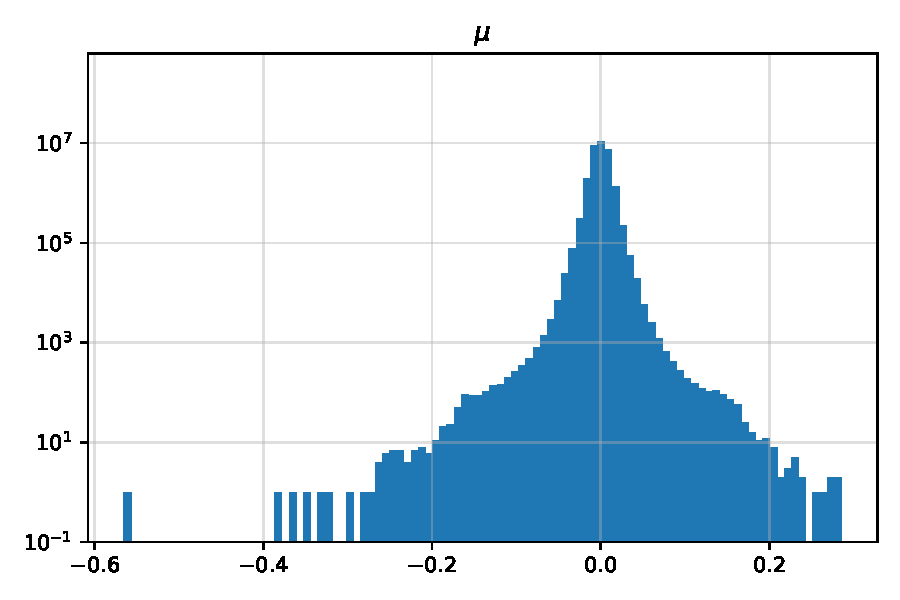
\includegraphics[width=0.6\linewidth]{images/weight/bcnn_rn_t1_lt5}
	\caption{Parameter value distribution of RainNet trained with one leadtime and Gaussian NLL $\sigma = 1e^{-4}$ after training. Histogram with 100 bins.}
	\label{fig:rn-weight}
\end{figure}

The first hyperparameter to be optimized for the Bayesian CNN is the prior. Here, it was chosen based on validation Gaussian NLL loss at model convergence. To give an idea about the natural distribution of network parameters under no regularizing prior, the parameter distribution for the deterministic RainNet with $\sigma = 1e^{-4}$ is shown in Figure \ref{fig:rn-weight}. The distribution is centered at 0 and has high kurtosis, mostly containing parameter values between  $-0.2$ and $0.2$. 


\begin{figure}[H]
	\centering
	\subfloat[Prior choice]{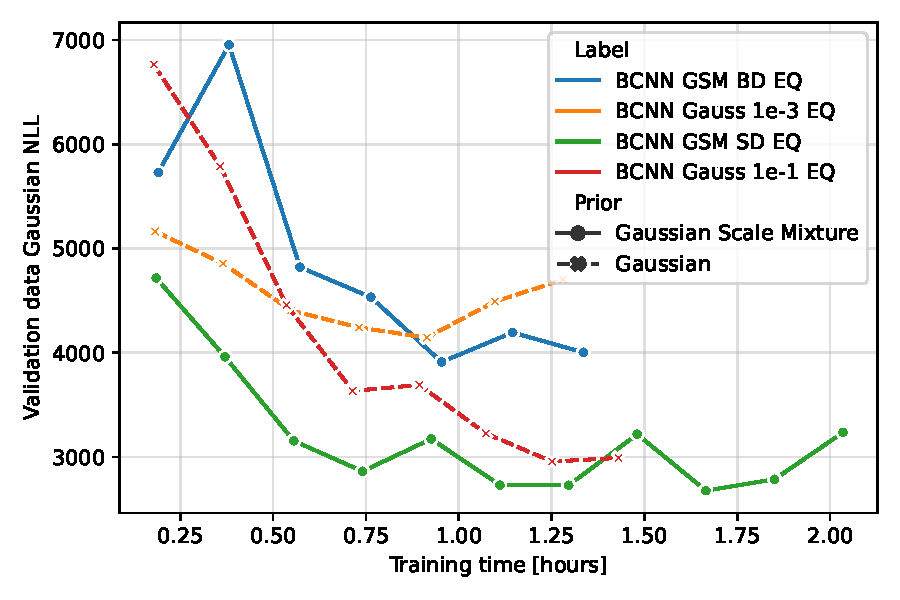
\includegraphics[width=0.33\linewidth]{images/model_choice/Prior_choice}}
	\subfloat[KL weighting choice]{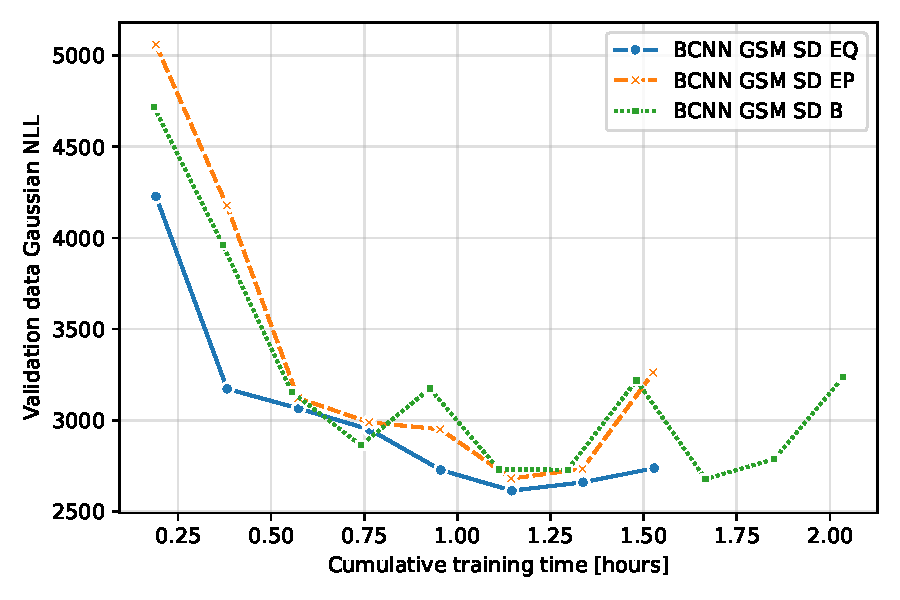
\includegraphics[width=0.33\linewidth]{images/model_choice/KL_weight_choice}}
	\subfloat[lt5 vs lt30]{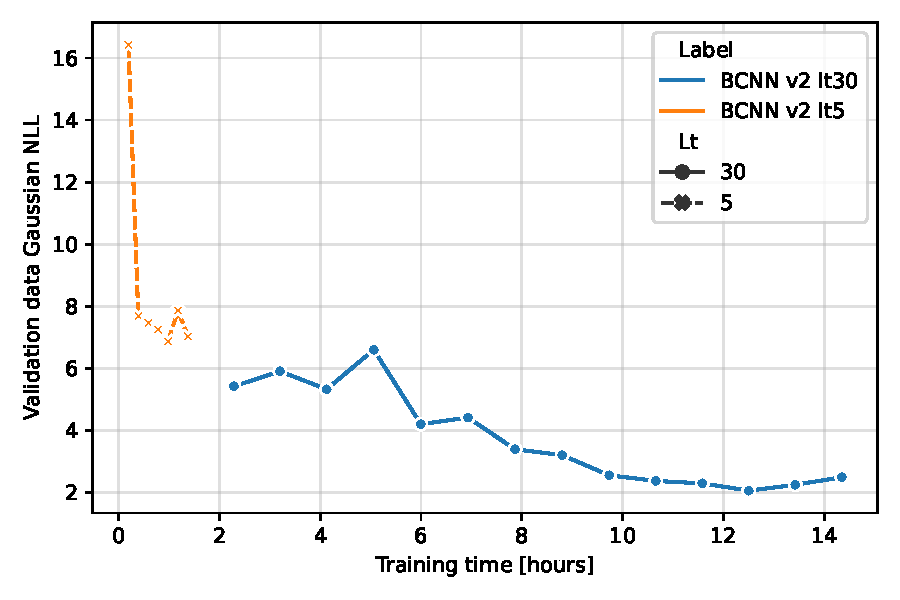
\includegraphics[width=0.33\linewidth]{images/model_choice/t3_training}}
	\caption{The validation set Gaussian NLL loss of the different BCNN candidates against total training time, highlighting the model selection process.}
	\label{fig:convergence-bcnn}
\end{figure}

Four priors were used as candidates based on knowledge of the "natural" parameter distribution. Two are Gaussian $\sim \mathcal{N}(0,1e^{-1})$ : \texttt{BCNN Gauss 1e-1 EQ}(1) and $\sim \mathcal{N}(0,1e^{-3})$: \texttt{BCNN Gauss 1e-3 EQ} (2); and two are Gaussian Scale Mixtures with $\sigma_1,\sigma_2 = 1e^{-1}, 1e^{-3}$ : \texttt{BCNN GSM BD EQ} (3) and $\sigma_1,\sigma_2 = 3e^{-1}, 3e^{-2}$ : \texttt{BCNN GSM SD EQ} (4). Prior (1) serves as a weak prior, allowing most "natural" parameter values. Prior (2) on the other hand is much stricter, restricting the range of possible values to be much smaller than it would be without it. Prior (3) mixes (1) and (2) to try to figure out if the approach of scale mixture has benefits. Prior (4) finally is based on the observation that the empirical distribution of deterministic RainNet models is relatively close the PDF of this prior, making it interesting to look at whether using it results in performance improvements.

The results of the optimization are shown in Figure \ref{fig:convergence-bcnn}.a. Here the KL-weighting scheme is set to equal weighting and the likelihood $\sigma = 1e^{-4}$. It is shown that that best performance is achieved by prior (4), making it the choice to be used in later experiments. The weaker prior (1) is slower to converge but achieves relatively good asymptotic performance, while the stricter prior (2) gives decent results more quickly but has trouble converging to low loss values. This was substantiated by prior (2) making blurrier forecasts. Prior (3) behaved as a middle-ground between priors (1) and (2). It benefited from the same fast initial convergence as prior (2) but achieved asymptotic performance somewhere between the two. 

\begin{figure}[H]
	\centering
	

	\subfloat[Gaussian prior $\sim \mathcal{N}(0,1e^{-1})$]{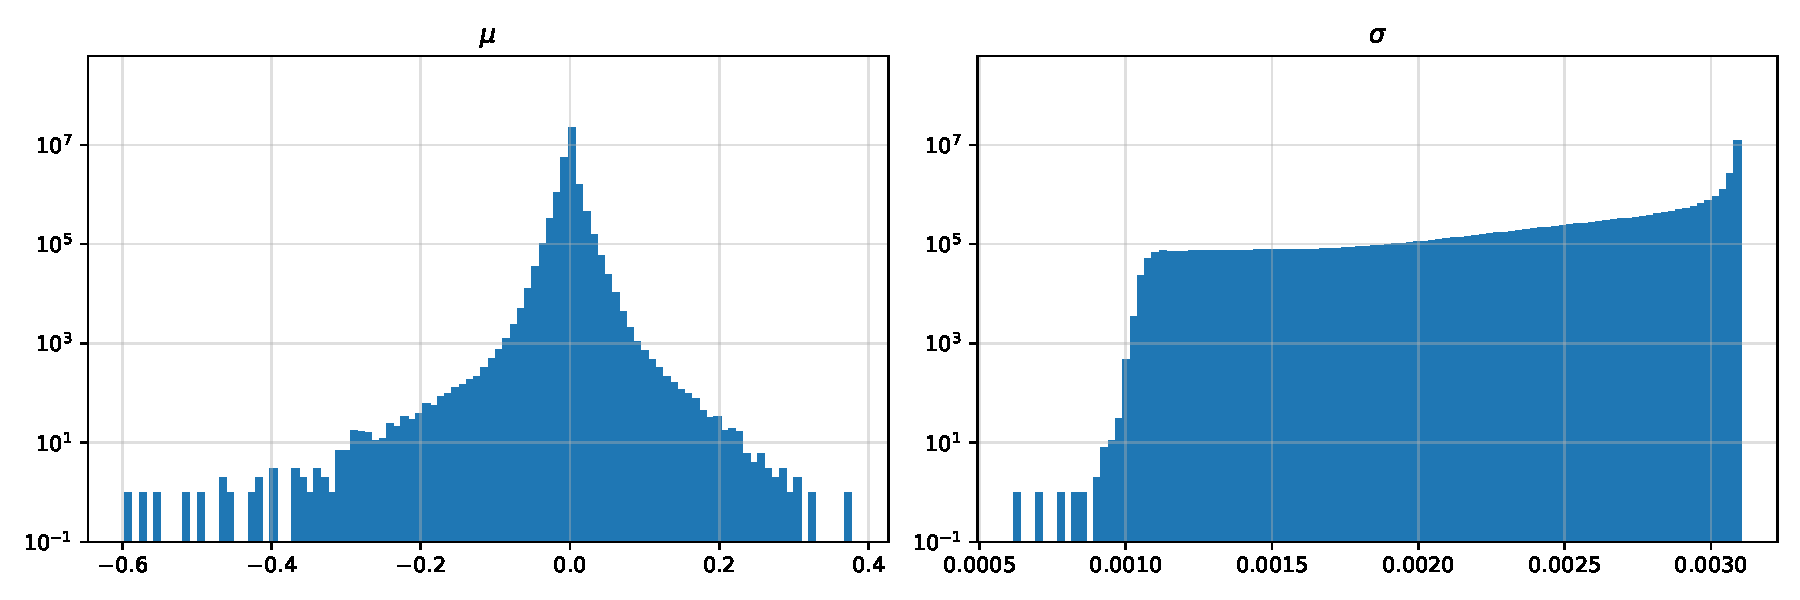
\includegraphics[width=0.5\linewidth]{images/weight/bcnn_t2}}
	\subfloat[Gaussian prior $\sim \mathcal{N}(0,1e^{-3})$]{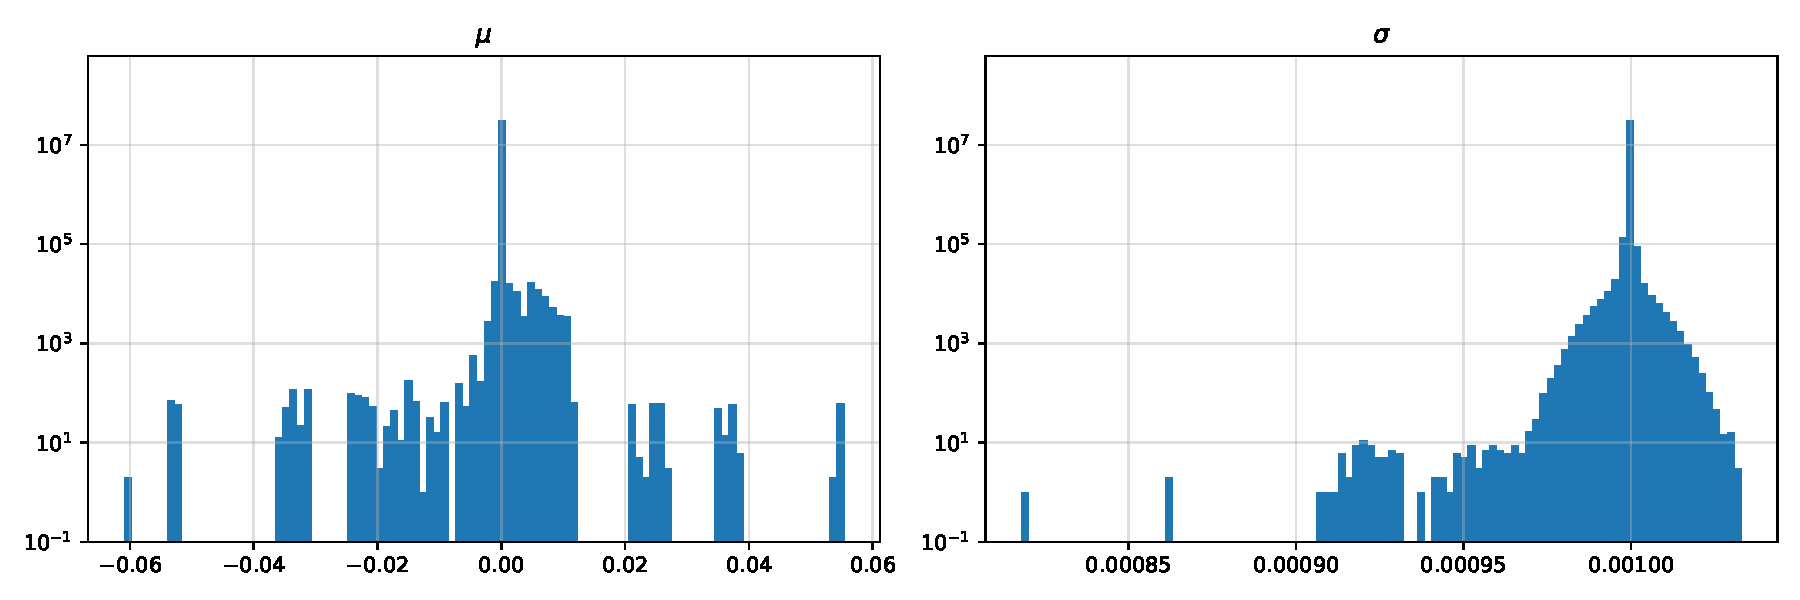
\includegraphics[width=0.5\linewidth]{images/weight/bcnn_t2_g_e-3}}
	

	\subfloat[Gaussian Scale Mixture Prior:\\ $\sigma_1,\sigma_2 = 1e^{-1}, 1e^{-3}$ ]{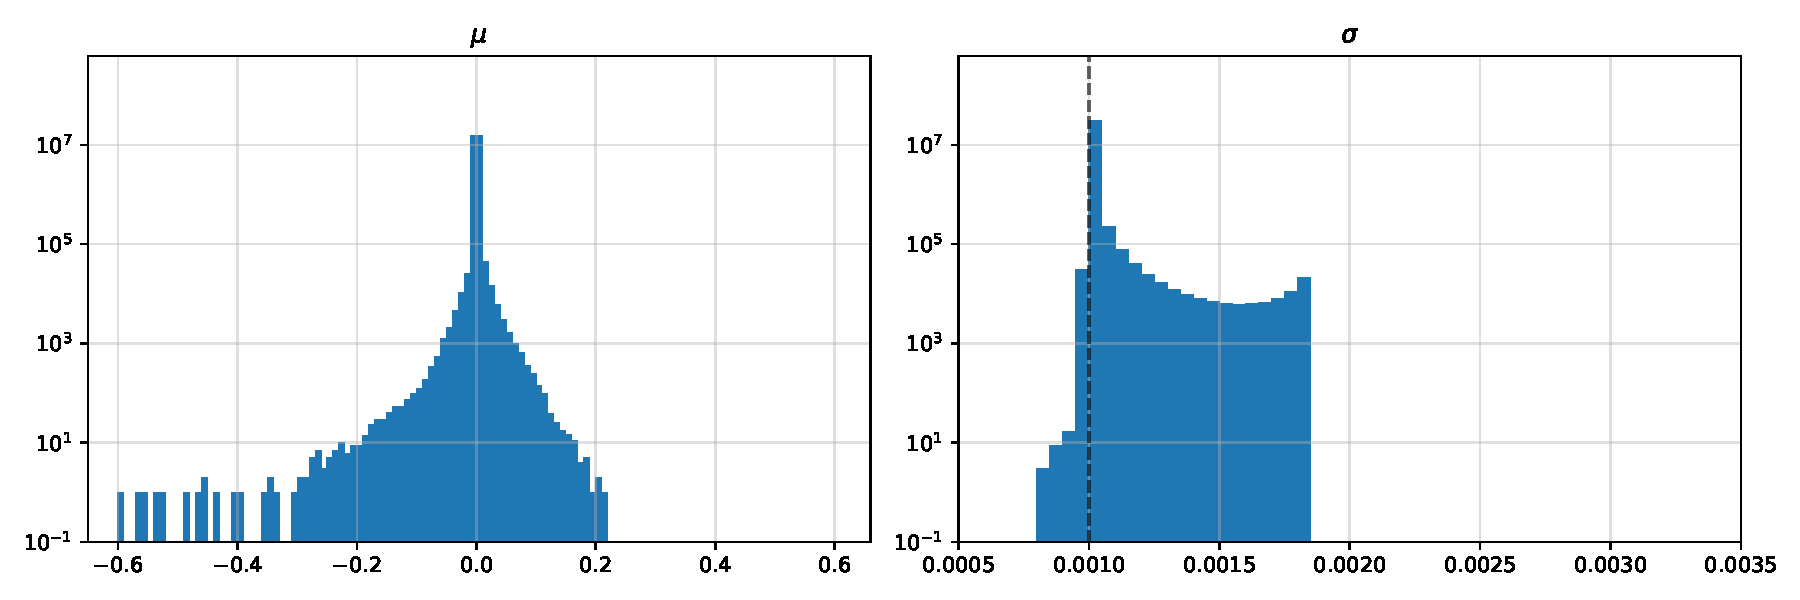
\includegraphics[width=0.5\linewidth]{images/weight/bcnn_t2_gsm_big_diff_lt5}}
	\subfloat[Gaussian Scale Mixture Prior:\\ $\sigma_1,\sigma_2 = 3e^{-1}, 3e^{-2}$]{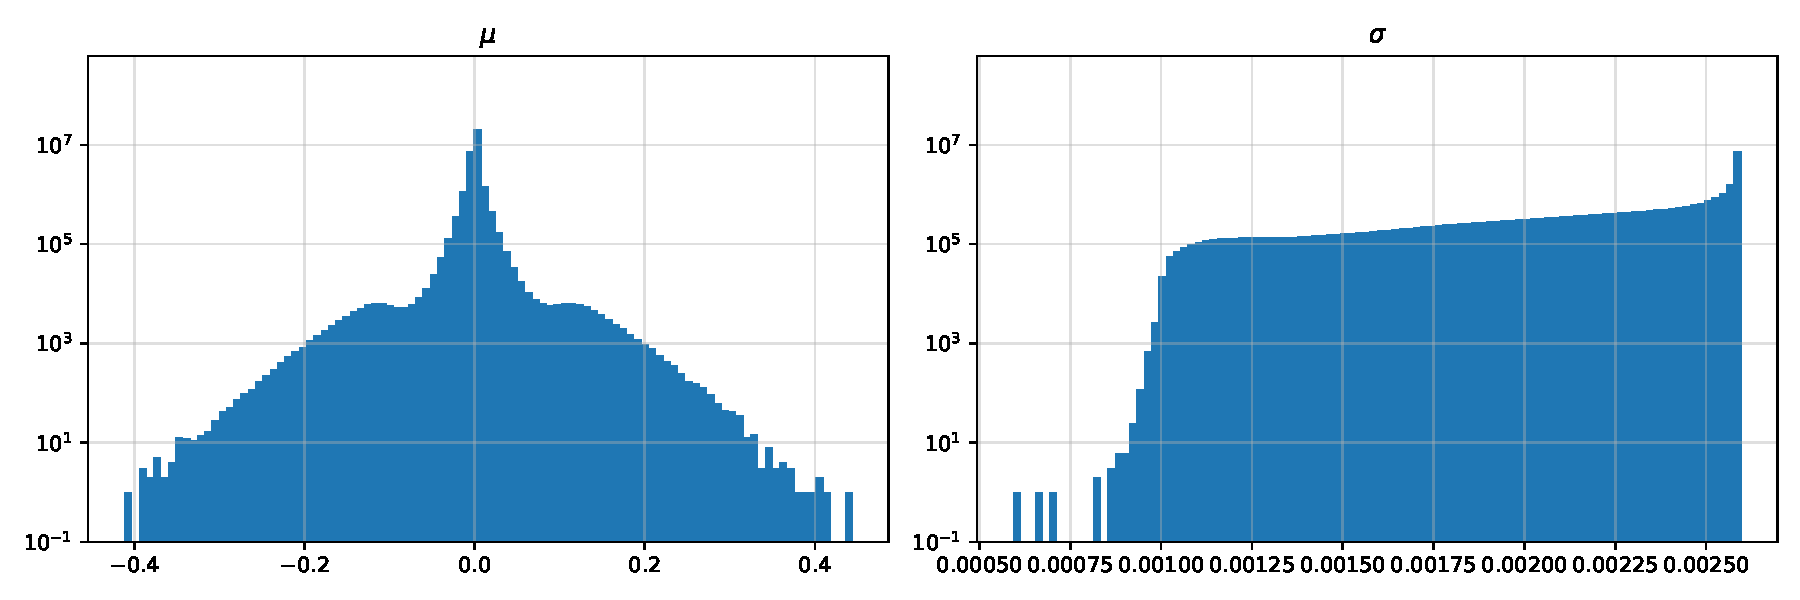
\includegraphics[width=0.5\linewidth]{images/weight/bcnn_t2_gsm_small_diff_lt5}}
	
	\caption{Final parameter posterior distributions in relation to the initial prior distribution chosen. $\mu$ histograms describe the parameter mean distributions, whereas $\sigma$ distributions describe the distribution of their standard deviations. The KL-weighting scheme here is set to equal weighting.}
	\label{fig:bcnn-prior-weights}
\end{figure}

The effect of the prior on the parameter mean and STD distributions is portrayed in Figure \ref{fig:bcnn-prior-weights}. It is seen that for all priors except (2), STD distributions end up tilted towards bigger values than the initial scale 1e-3, pointing to a possibility that it was way too small and that combined with a small learning rate 1e-4, there wasn't just enough time for the them to grow where they should have. Concerning means, it is observed that the breadth of the posterior mean distribution is closely associated to the prior distribution breadth. With prior (2), it is seen that, most means are actually very close to 0 and while scales are close to their initial values, the biggest deviations tend to lower them, which can be intuitively understood as the prior scale is the same as the initial posterior scale.  

With the prior chosen, the next hyperparameter to be optimized is the KL weighting scheme. \texttt{BCNN GSM SD EQ} refers to the \texttt{equal} weighting scheme, \texttt{BCNN GSM SD EP} to the \texttt{epoch} weighting scheme, and \texttt{BCNN GSM SD B} to the \texttt{blundell} weighting scheme. The results are depicted in Figure \ref{fig:convergence-bcnn}.b. Best performance is observed with the Blundell weighting scheme which was chosen for further experiments, with close performance achieved using equal weighting. Although relatively close in performance, the Epoch weighting scheme did not deliver in the end, although it showed promising results in preliminary experiments, where the Blundell scheme did not work. The effect of the KL weighting scheme on the weight distribution is shown in Figure \ref{fig:bcnn-training-weights}. Here, the Blundell scheme differs considerably compared to others in terms of scale distribution, as they are more closely centered around the initial value and the shift is directed towards smaller values. 

Finally total cumulative training times for \texttt{lt5} and \texttt{lt30} variants are compared in Figure \ref{fig:convergence-bcnn}.c. The training are shown for the model \texttt{BCNN lt5 V2}, which is an additional experiment not used for other verification. It is seen that continuing the training with 30 minute leadtime, i.e. six predictions, requires much more computational resources than simply using 5 minute leadtime, i.e. one prediction, which is only worth if skill is improved as a result. In the current example, using a likelihood $\sigma$ parameter of 2e-2, likelihood loss is improved with \texttt{lt30}, but the opposite is found using a likelihood $\sigma$ of 1e-4.

\section{Nowcasting Examples}

Here, example nowcasts made with the developed model are shown for two distinct events. The main three models retained for verification are \texttt{BCNN lt5}, \texttt{BCNN lt30}, \texttt{BCNN lt5 new}. The main model showcased is \texttt{BCNN lt5}, with additional models showcases as well as results for STEPS in Appendix \ref{section:additional-case-studies}.  Predictive mean and uncertainty, as well as exceedance probabilities for 0.5, 5.0, and 20.0 mm/h are shown.  

\subsection{Case Study 1 : Rapidly Moving Mixed Stratiform and Convective Rain Event}

\begin{figure}[H]
	\centering
	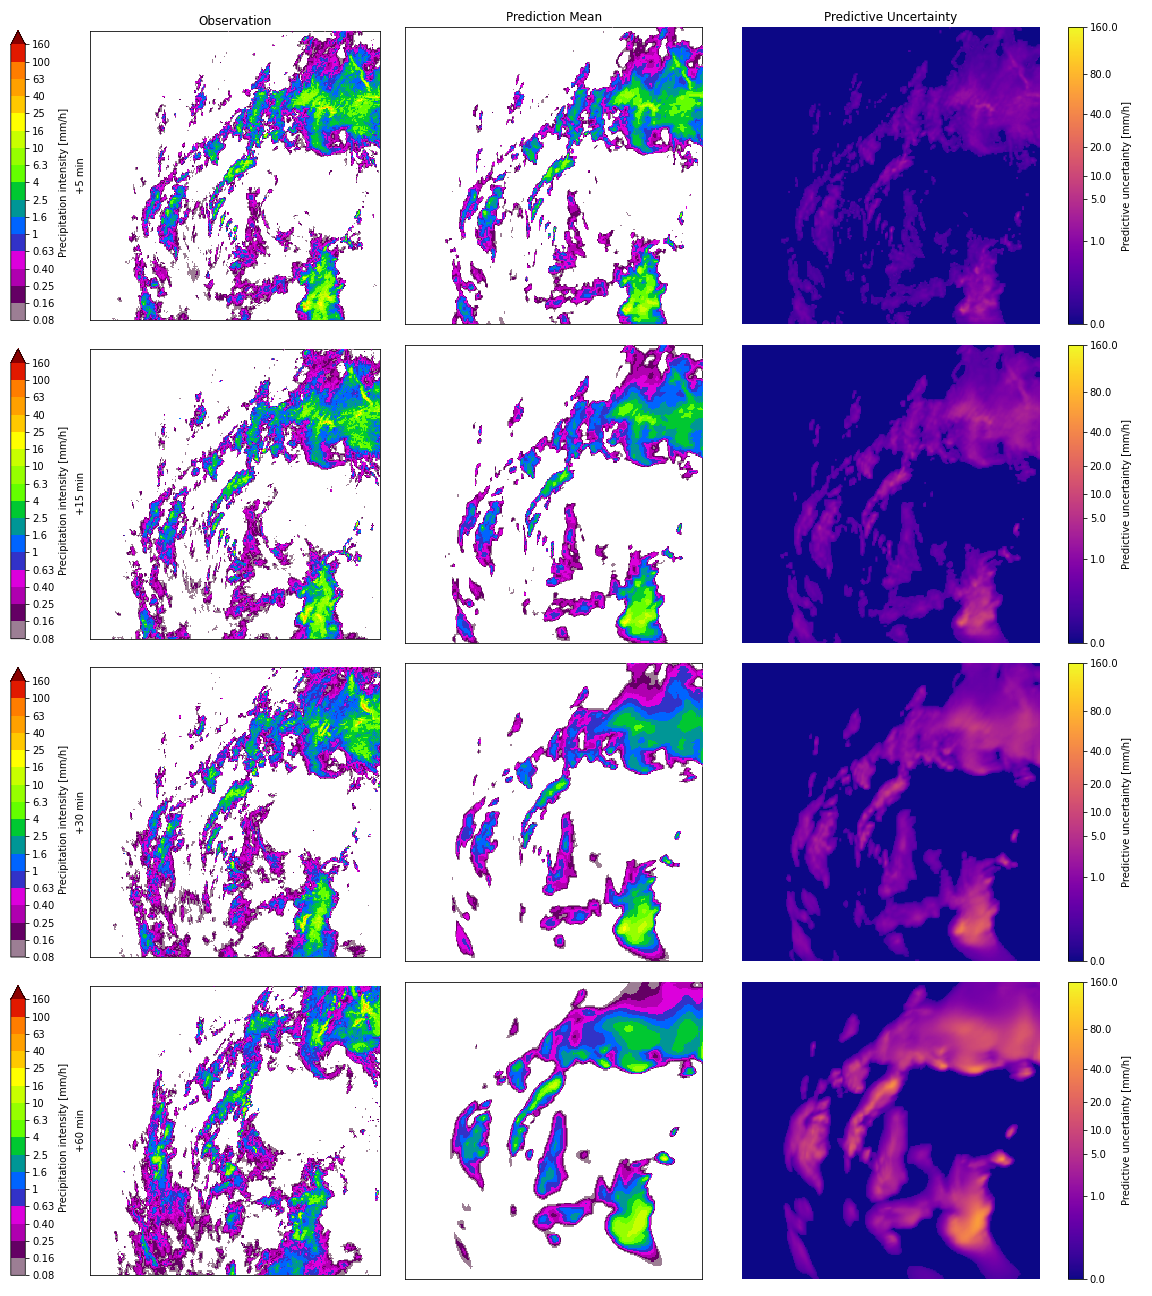
\includegraphics[width=\textwidth]{images/cases/bcnn_mean_case1}
	\caption{Predictive mean and uncertainty (two standard deviations) for Case 1 on the 25th of May 2019 starting at 13:00 local Helsinki time for the \texttt{BCNN lt5} model, covering the area of southern Finland.}
	\label{fig:bcnn_mean_case1}
\end{figure}

The predictive mean and uncertainty for \texttt{BCNN lt5} on Case 1 is shown in Figure \ref{fig:bcnn_mean_case1}. It is observed that mean predictions get increasingly smoothed out with time as expected, and that predictive uncertainty is highly correlated with predicted mean rainrate. 
%
%
Additionally, predictive uncertainty increases over time, achieving top values exceeding 50 mm/h in areas of predicted heavy rain at one-hour leadtimes. It is seen that advection and the overall movement of the front is well-modeled, while smaller-scale details even if corresponding to medium or heavy rain, are quickly lost. 



Smoothing out of predictions has an important effect of reducing model capacity to predict high rainrates, which are often concentrated over small areas. This is an especially important effect because smoothing does not originate simply from averaging, but is also present in individual ensemble members, due to the combined effect of the loss function and of the iterative prediction scheme, as described in Section \ref{section:rainnet}. 

\begin{figure}[H]
	\centering
	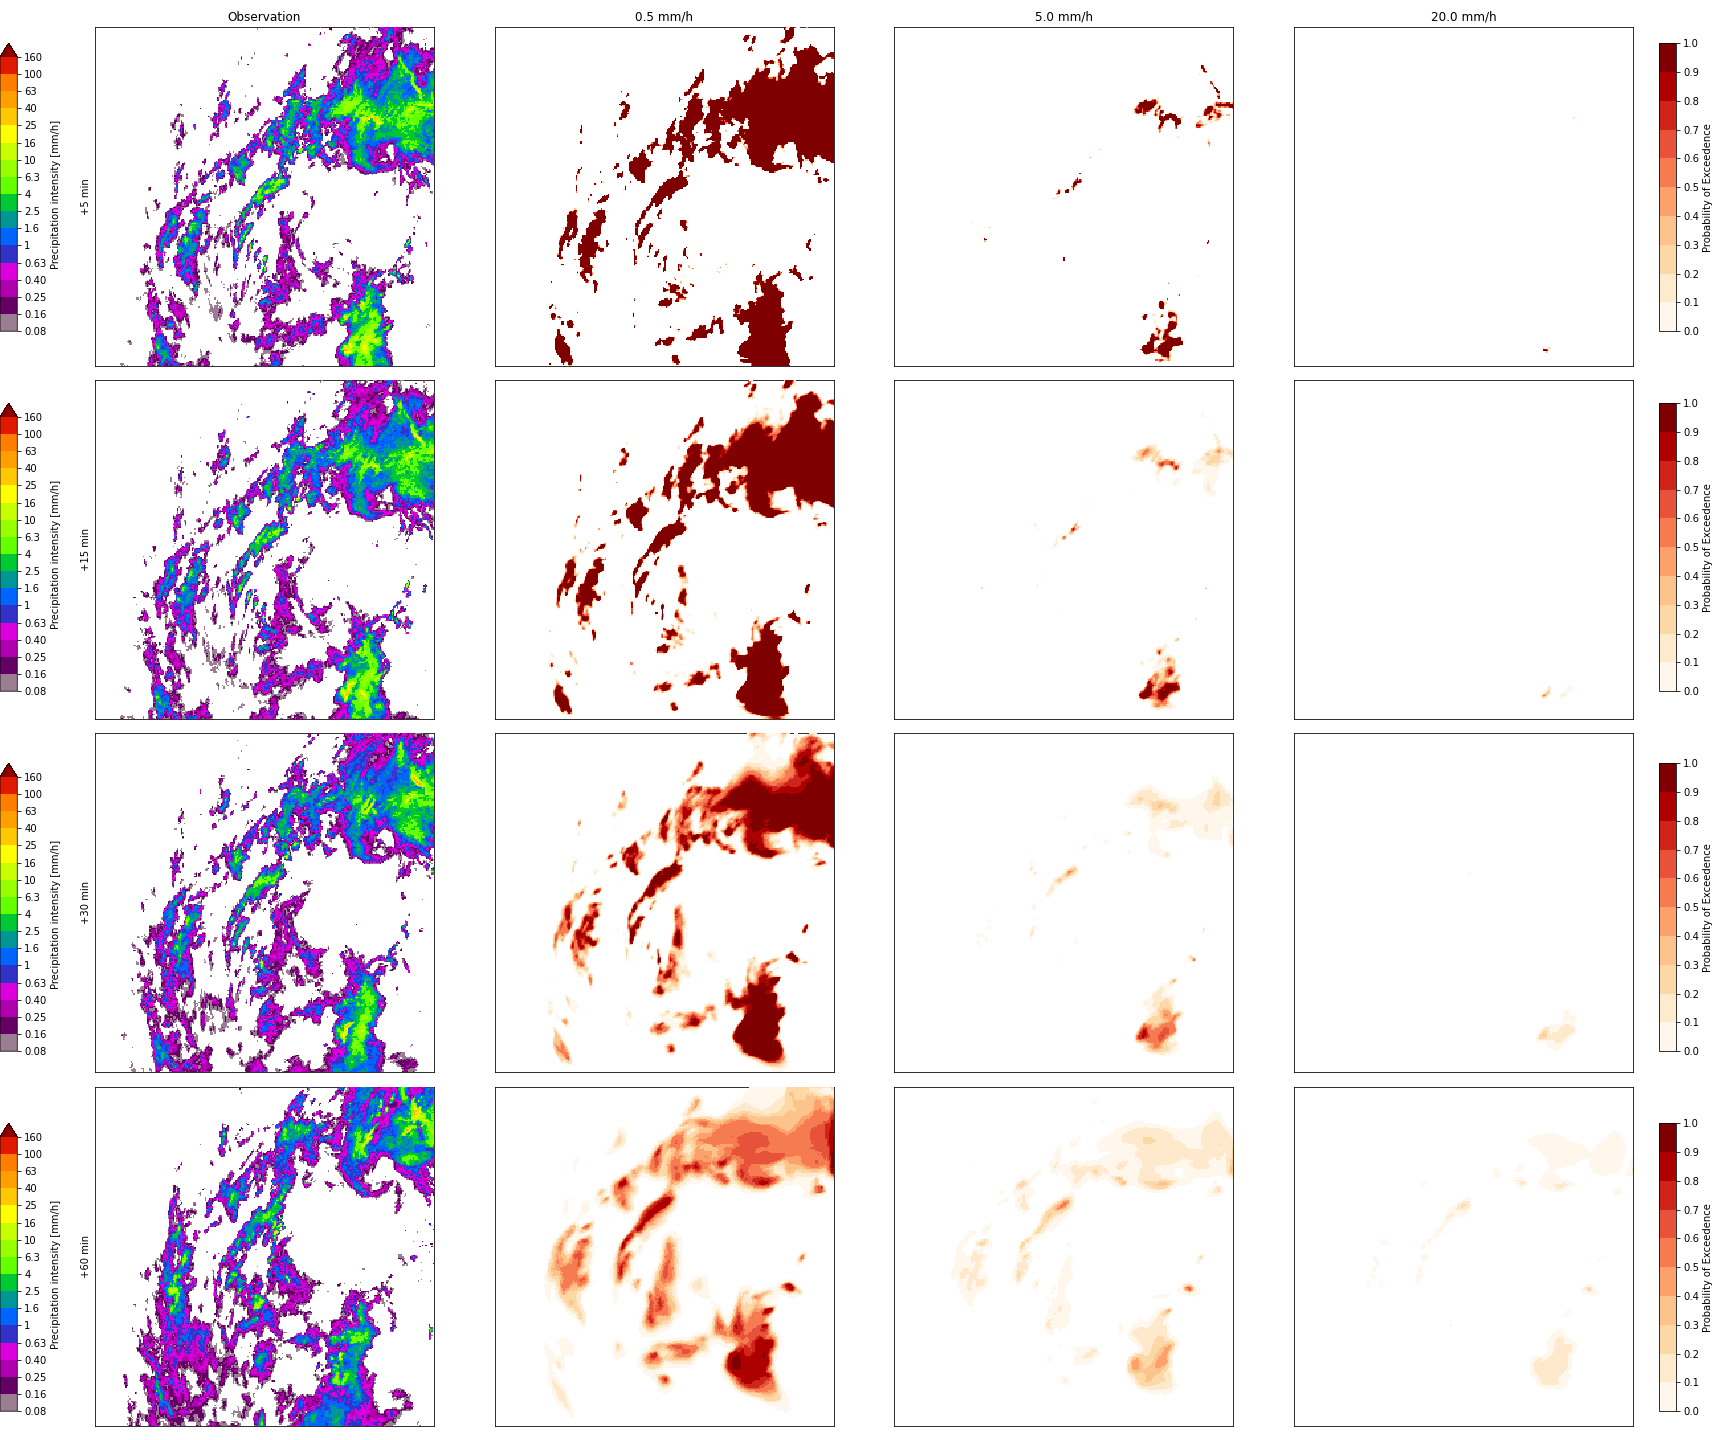
\includegraphics[width=\textwidth]{images/cases/bcnn_prob_case1}
	\caption{0.5, 5.0, and 20.0 mm/h exceedance probabilities for Case 1 on the 25th of May 2019 starting at 13:00 local Helsinki time for the \texttt{BCNN lt5} model, covering the area of southern Finland.}
	\label{fig:bcnn_prob_case1}
\end{figure}

Exceedance probabilities for \texttt{BCNN lt5} on Case 1 are shown in Figure \ref{fig:bcnn_prob_case1}. Both for this model and in general, it is seen that exceedance probabilities are lower for high leadtimes and high thresholds. In the case of this model, all exceedance probabilities seem to be smoothed over time, which is indicative of the uncertainty of the extent of rain being at least to some degree taken into account. It is also seen that especially at 20.0 mm/h, the predicted exceedance probability at one-hour leadtime does not always originate from current time high rainrates. This is seen from the top of the image at +5min, where a small exceedance probability is present, but disappears at further leadtimes, before reappearing independently. 



Both in the plot of prediction mean and uncertainty, as well as in that of exceedance probabilities, it is seen that because the rain is advected towards the north, lower parts of the image can not be predicted. 

\subsection{Case Study 2 : Mixed Stratiform and Convective Rain Event with Spinning Motion}

The predictive mean and uncertainty for \texttt{BCNN lt5} on Case 2 is shown in Figure \ref{fig:bcnn_mean_case2}. In this case, the same overall features are observed as in Case 1. Here, the spinning motion is correctly predicted and the mean rainrates are relatively close to ground truth. As in Case 1 but especially here, many small features are lost and especially small convective cell evolution is not correctly predicted. 

\begin{figure}[H]
	\centering
	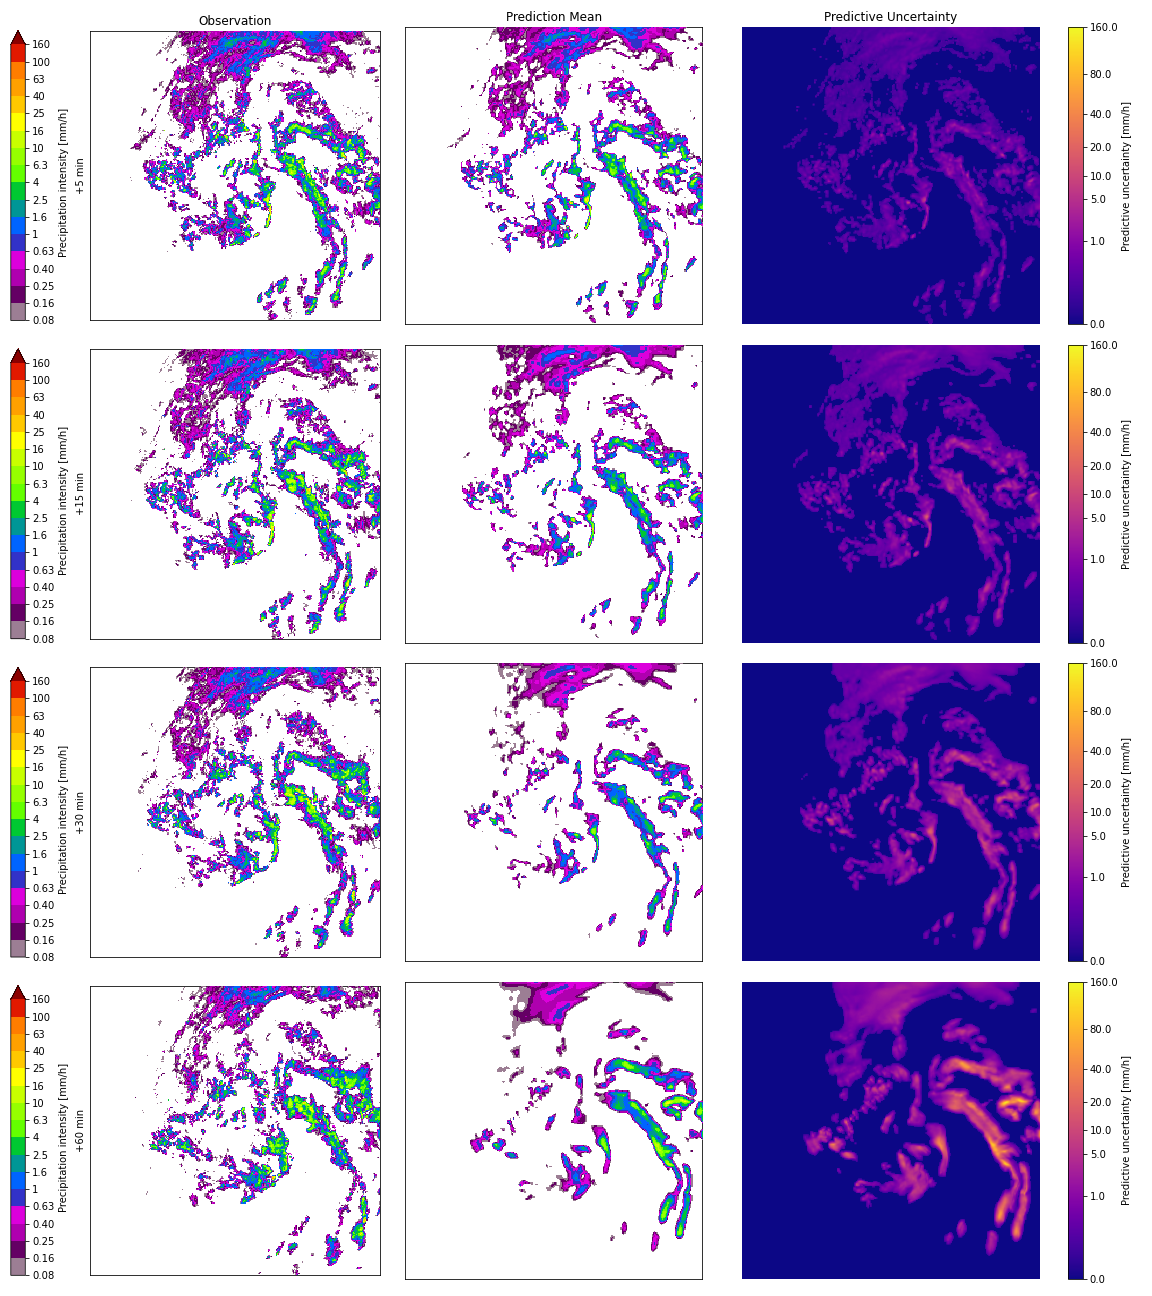
\includegraphics[width=\textwidth]{images/cases/bcnn_mean_case2}
	\caption{Predictive mean and uncertainty (two standard deviations) for Case 2 on the 18th of May 2021 starting at 21:00 local Helsinki time for the \texttt{BCNN lt5} model, covering the area of southern Finland.}
	\label{fig:bcnn_mean_case2}
\end{figure}

The exceedance probabilities are shown in Figure \ref{fig:bcnn_prob_case2}. Many things happening here are similar to Case 1, but especially striking is lower exceedance probabilities at one-hour leadtime for the 0.5 mm/h threshold. Here, in many samples the spinning "arms" were lost by that time because of their thinness and the tendency of thin or small features to disappear. 

\begin{figure}[ht]
	\centering
	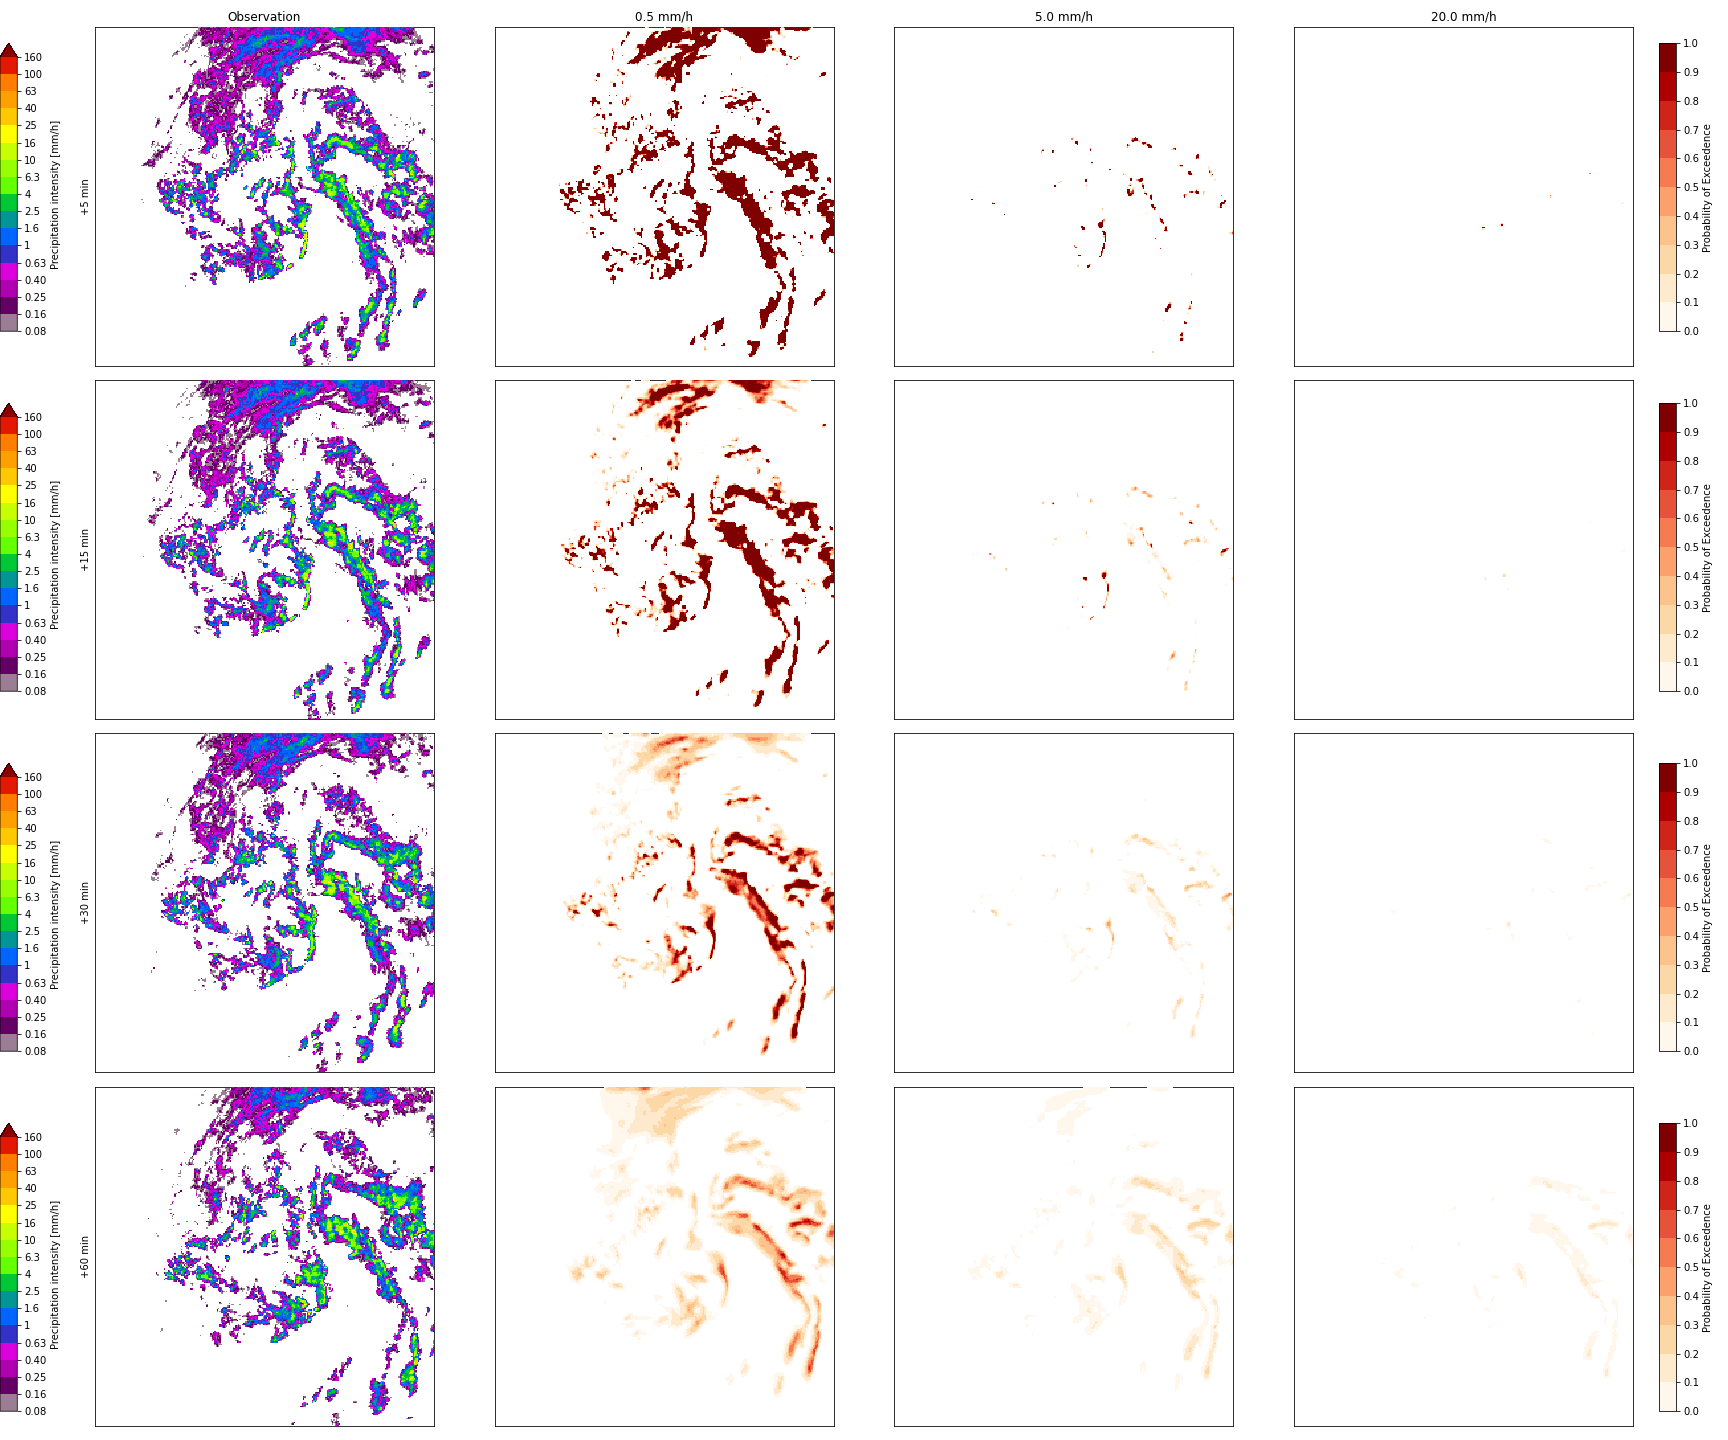
\includegraphics[width=\textwidth]{images/cases/bcnn_prob_case2}
	\caption{0.5, 5.0, and 20.0 mm/h exceedance probabilities for Case 2 on the 18th of May 2021 starting at 21:00 local Helsinki time for the \texttt{BCNN lt5} model, covering the area of southern Finland.}
	\label{fig:bcnn_prob_case2}
\end{figure}

\subsection{Additional Case Study 1 Results}

Case 1 prediction mean and uncertainty, as well as exceedance probabilities are respectively plotted for \texttt{BCNN lt5 new} in Figures \ref{fig:bcnn_better_mean} and \ref{fig:bcnn_better_prob}, \texttt{BCNN lt30} in Figures \ref{fig:bcnn_p2_lt30_mean} and \ref{fig:bcnn_p2_lt30_prob}, and finally STEPS in Figures \ref{fig:steps_mean} and \ref{fig:steps_prob}. For \texttt{BCNN lt5 new}, results are similar as in the \texttt{BCNN lt5} case, but exhibit a much bigger bias towards predicting strong rain, with more ensemble members predicting increasingly high rainrates. From exceedance probabilities, this can be seen as overall higher values, making the model more susceptible to predicting stronger rainrates. 

For \texttt{BCNN lt30}, it can be seen from both figures that the overall skill is lower than for \texttt{lt5} cases. In particular, predictions are more smoothed out and more details are lost, hinting to the conclusion that \texttt{lt30} training did not work as expected. Here, predictive uncertainty does not increase with leadtime, and higher rainrates are often not predicted at all. However it can be seen that the network predicts consistently high exceedance probabilities, and that those are not (esp. 0.5 mm/h) smoothed out spatially with increased leadtime. 

Finally, looking out at figures of the STEPS baseline, it is easily seen that despite being a simpler model, it predicts better spatial uncertainty in future rain. However STEPS has a hard time predicting exceedance probabilities for high (esp. 20.0 mm/h) thresholds. One striking feature is also that in the case of STEPS, predictive uncertainty is more spread out than predictive mean, which is a behavior not observed in any model developed here. 


\section{Deterministic Prediction Skill}

The following results describe the skill of ensemble means of developed models against baseline models.% LINDA-P ensemble means are omitted for clarity because their skill was almost identical to LINDA-D. 

\begin{figure}[H]
	\centering
	\subfloat[MAE]{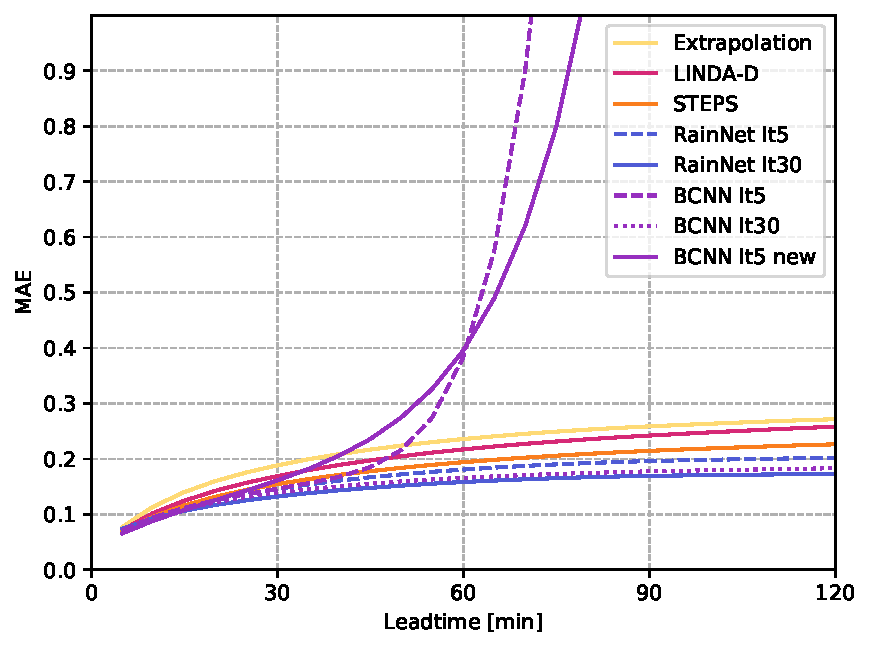
\includegraphics[width=0.5\textwidth]{images/metrics/ALL_MAE}}%
	\subfloat[ME]{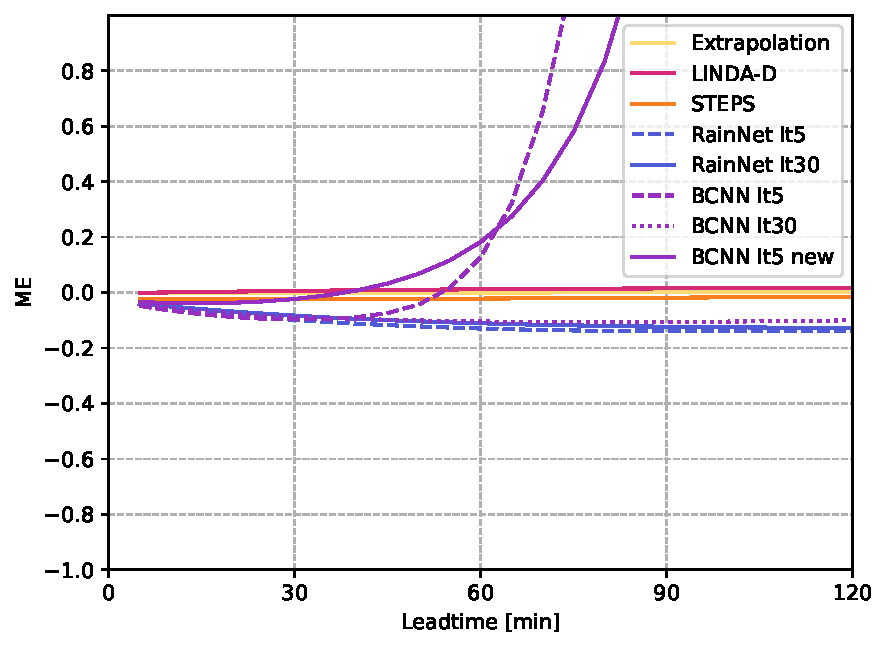
\includegraphics[width=0.5\textwidth]{images/metrics/ALL_ME}}%

	\caption{Continuous Metrics (MAE and ME) for BCNN variants and baselines, up until two-hour leadtime.}
	\label{fig:cont-metrics}
\end{figure}

Starting off with the continuous metrics, their values are shown in Figure \ref{fig:cont-metrics}. BCNN and RainNet models have similar MAE and ME, except for \texttt{BCNN lt5} and \texttt{BCNN lt5 new} cases, where ensemble means exhibited clear bias towards too strong rainrate predictions after 30 minutes. These models shall be called "positively biased". ME was around zero for classical models and tended lower with other RainNet and BCNN models, showing bias towards too weak predictions ("negatively biased"), mainly due to smoothing. Still, BCNN and RainNet gave mostly clearly superior MAE compared to classical models, which is understandable as Gaussian NLL is a loss function part of the same class as MAE, which tends to optimize for minimizing pixel-per-pixel deviations and by extension MAE. 

\begin{figure}[H]

	\centering
	\subfloat[ETS 0.5 mm/h]{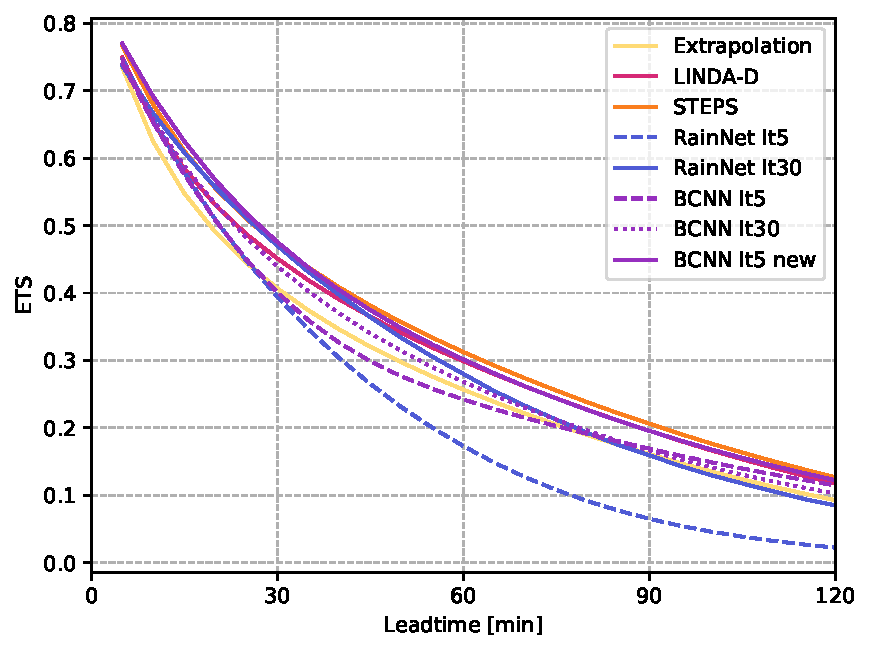
\includegraphics[width=0.35\textwidth]{images/metrics/ALL_ETS_0_5}}%
	\subfloat[ETS 5.0 mm/h]{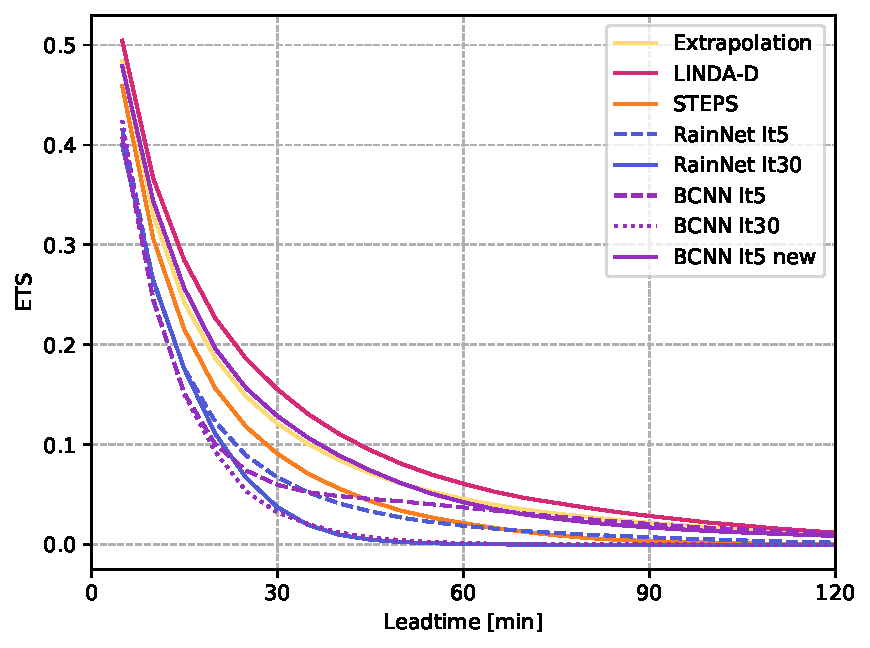
\includegraphics[width=0.35\textwidth]{images/metrics/ALL_ETS_5_0}}%
	\subfloat[ETS 20.0 mm/h]{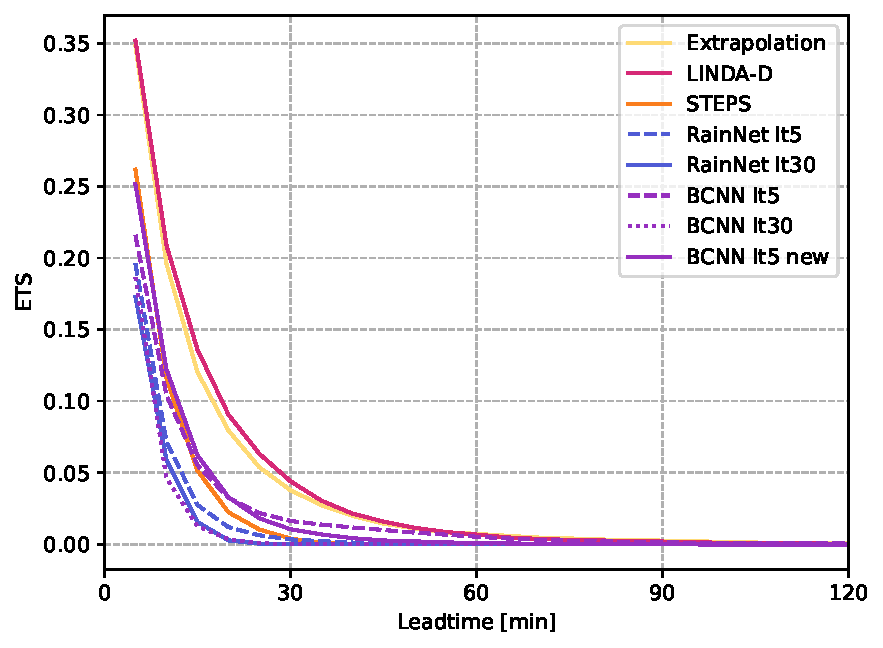
\includegraphics[width=0.35\textwidth]{images/metrics/ALL_ETS_20_0}}%
	
	
	
	\subfloat[FAR 0.5 mm/h]{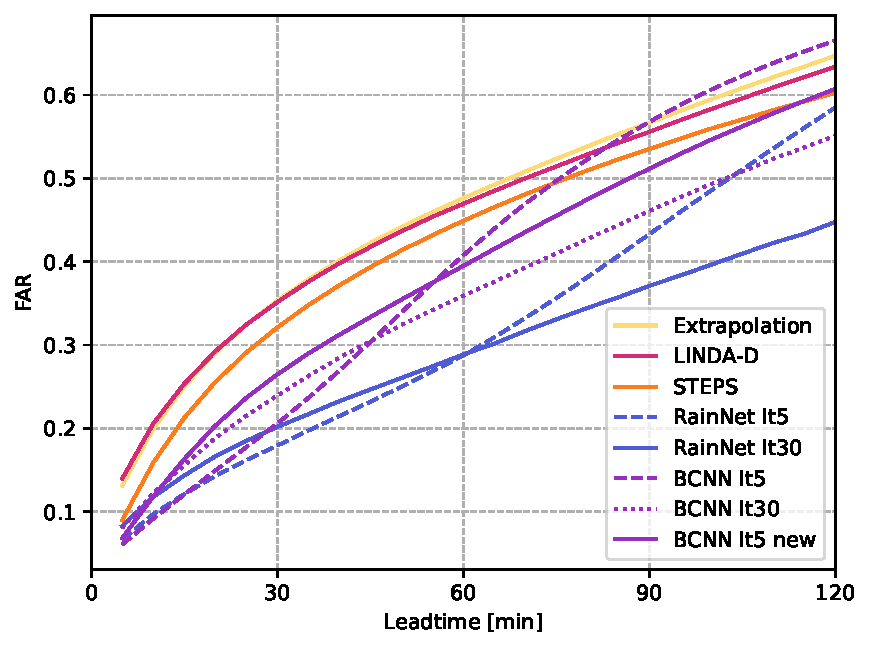
\includegraphics[width=0.35\textwidth]{images/metrics/ALL_FAR_0_5}}%
	\subfloat[FAR 5.0 mm/h]{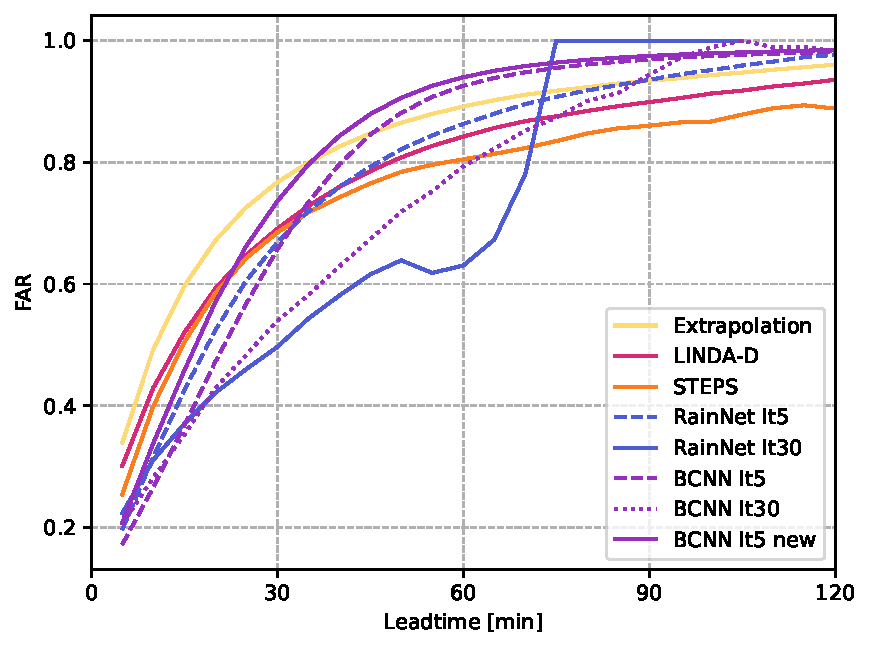
\includegraphics[width=0.35\textwidth]{images/metrics/ALL_FAR_5_0}}%
	\subfloat[FAR 20.0 mm/h]{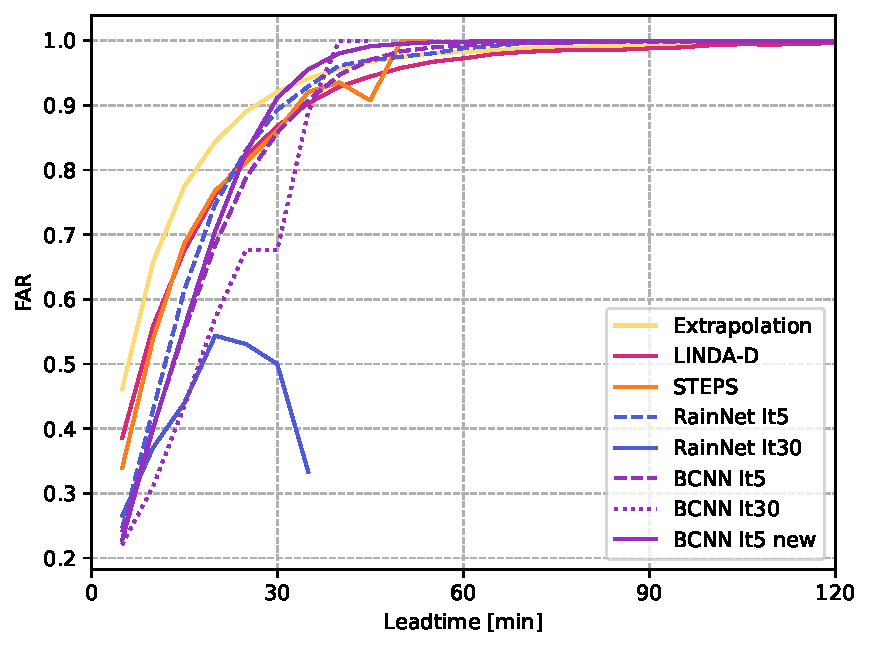
\includegraphics[width=0.35\textwidth]{images/metrics/ALL_FAR_20_0}}%
	
	\subfloat[POD 0.5 mm/h]{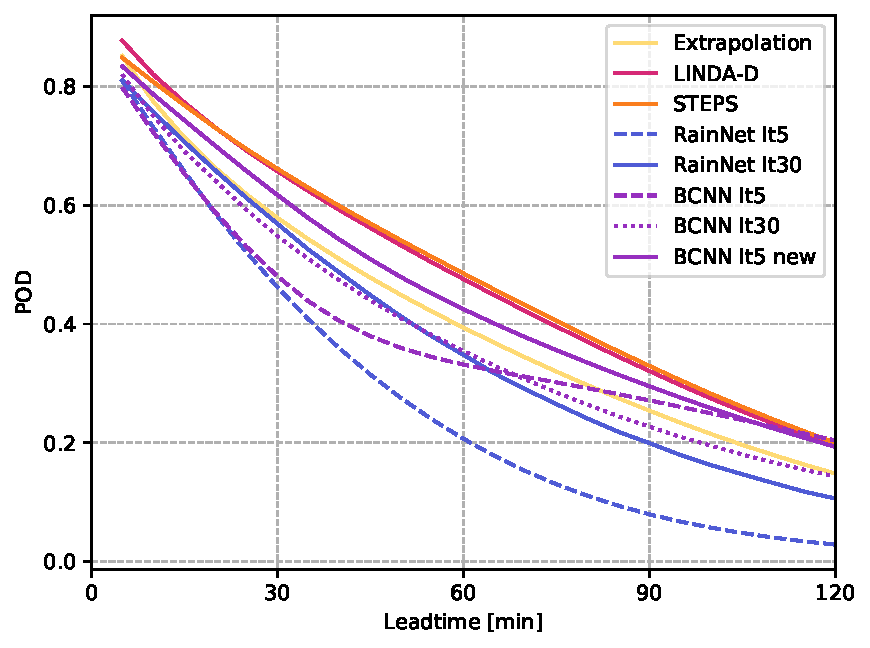
\includegraphics[width=0.35\textwidth]{images/metrics/ALL_POD_0_5}}%
	\subfloat[POD 5.0 mm/h]{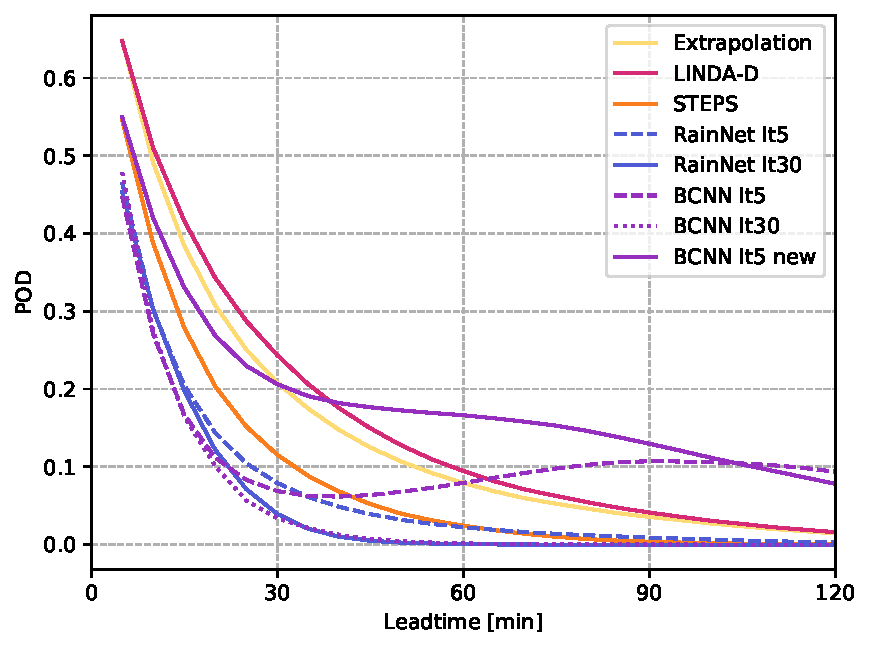
\includegraphics[width=0.35\textwidth]{images/metrics/ALL_POD_5_0}}%
	\subfloat[POD 20.0 mm/h]{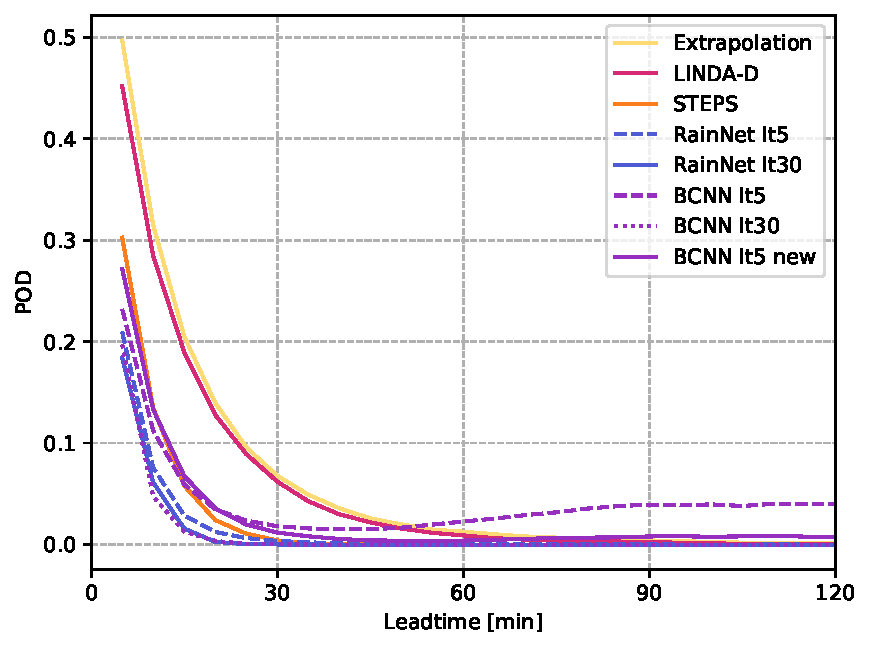
\includegraphics[width=0.35\textwidth]{images/metrics/ALL_POD_20_0}}%
	\caption{Categorical metrics (ETS. FAR, and POD) for BCNN variants and baselines, up until two-hour leadtime at thresholds of 0.5, 5.0, and 20.0 mm/h.}
	\label{fig:cat-metrics}
\end{figure}

POD, FAR, and ETS metric values are shown in Figure \ref{fig:cat-metrics}. For these metrics, the strongest overall result among developed models is achieved by \texttt{BCNN lt5 new}, which is strongly positively biased. 
%This is not unexpected, as positively biased models seem to perform better with categorical metrics than negatively biased. 
For POD, a resurgence at further leadtimes is seen in \texttt{BCNN lt5} and \texttt{BCNN lt5 new} models, because of the phenomenon of "exploding rainrates".  In other cases, POD is better for classical baselines than CNN based models, when negatively biased. Accompanying high POD of "exploding rainrates" of positively biased models is a very high FAR, demonstrating that this high POD is not necessarily indicative of skill. FAR is interestingly worse for extrapolation based baselines than CNN based models at 0.5 mm/h threshold, a phenomenon that disappears at higher thresholds.

 ETS summarizes the categorical skill of the models. Especially at 5.0 and 20.0 mm/h, LINDA-D has the best predictive skill, while CNN based models and STEPS lag far behind. Overall, no conclusion can be made about whether the Bayesian extension improved the categorical predictive skill, as the the only skillful outlier \texttt{BCNN lt5 new} didn't have a RainNet model with a corresponding training routine to compare to. CSI scores are shown in Figure \ref{fig:csi}, but they do not differ much from ETS. 

\begin{figure}[H]
	\subfloat[0.5 mm/h]{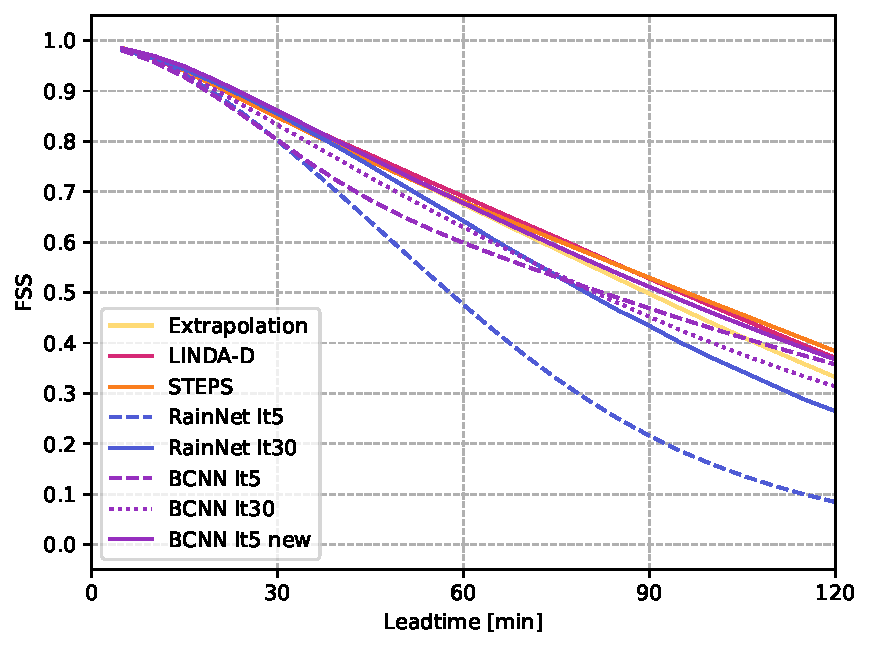
\includegraphics[width=0.33\textwidth]{images/metrics/ALL_FSS_8_0_5}}%
	\subfloat[5.0 mm/h]{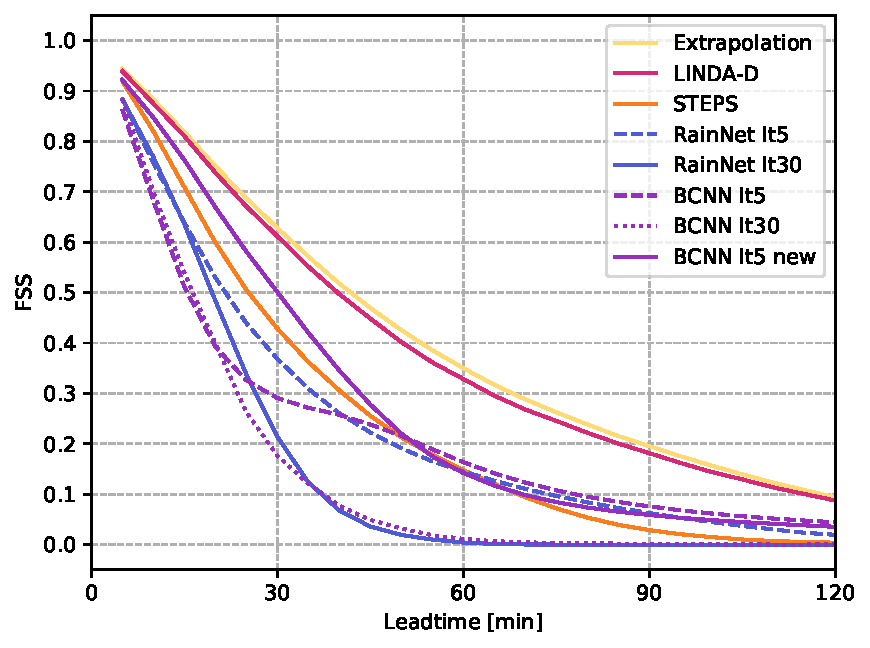
\includegraphics[width=0.33\textwidth]{images/metrics/ALL_FSS_8_5_0}}%
	\subfloat[20.0 mm/h]{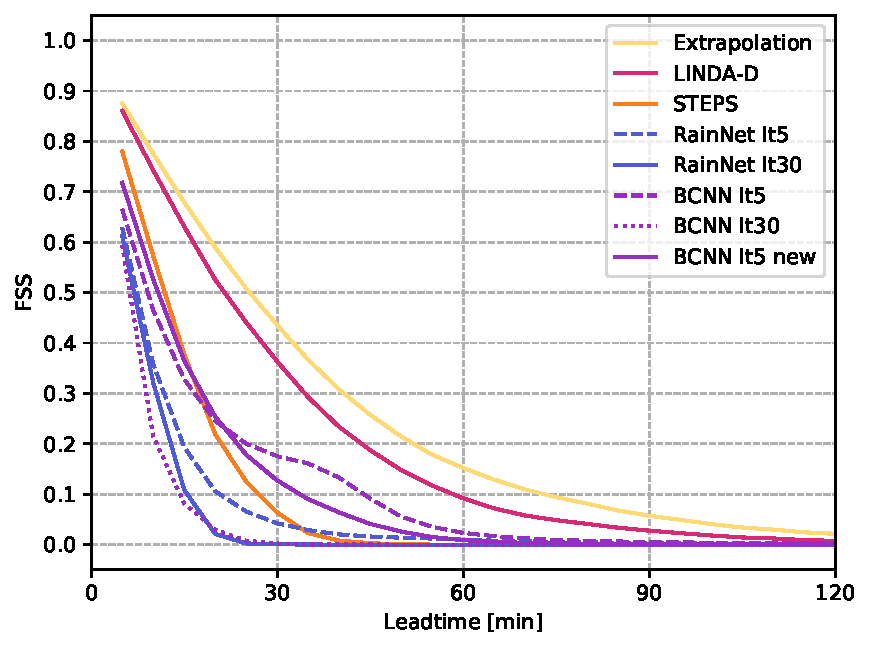
\includegraphics[width=0.33\textwidth]{images/metrics/ALL_FSS_8_20_0}}%
	\caption{FSS metric at a 16km scale for BCNN variants and baselines, up until two-hour leadtime at thresholds of 0.5, 5.0, and 20.0 mm/h.}
	\label{fig:fss16}
\end{figure}

The FSS metric results at a 16km spatial scale for the thresholds of interest are shown in Figure \ref{fig:fss16}. Here, it is found that the difference between extrapolation based deterministic models and others is strikingly big. FSS at a scale of 4km is shown in Figure \ref{fig:fss4}, but the results do not differ much from ETS and CSI at the original scale of two kilometers, as the change is only two-fold. 

RAPSD is shown in Figure \ref{fig:rapsd} for leadtimes of 15, 60, and 120 minutes. As expected, Extrapolation nowcast which preserves details has a PSD very close to observations, while other models show drop in power at short wavelengths, with steeper drops at further leadtime. Interestingly, this drop in power is bigger at 60 minutes than 120 minutes, which might have something to do with the OR-masking of NaN values, reducing significantly the area used for calculation at two hours. The biggest drops in small-scale details are experienced by STEPS and \texttt{BCNN lt30} as well as \texttt{RainNet lt30} models. All \texttt{lt5} CNN models experienced less loss in details compared to \texttt{lt30} models. It is difficult to conclude whether taking ensemble means had any significant effect on the loss of small-scale details of CNN approaches without looking at individual ensemble members and ditching the OR-masking.

\begin{figure}[H]
	\centering
	\subfloat[15 min]{
	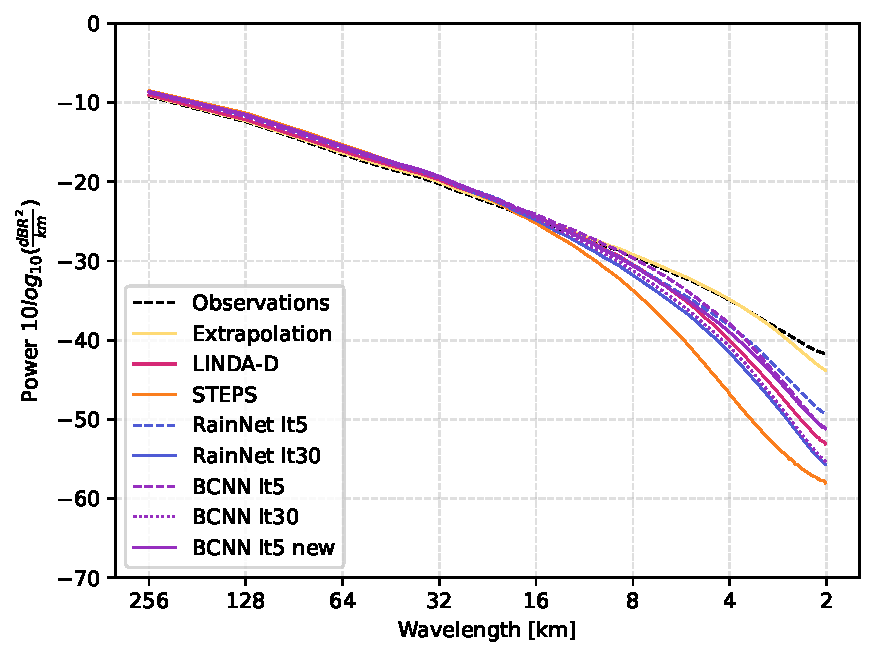
\includegraphics[width=0.33\textwidth]{images/metrics/ALL_15min_RAPSD}
}
	\subfloat[60 min]{
		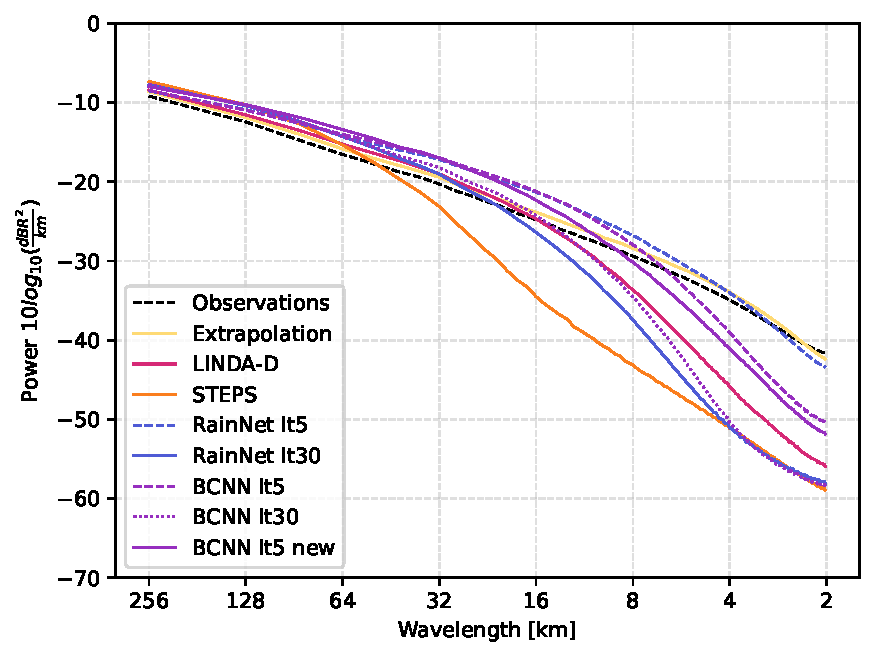
\includegraphics[width=0.33\textwidth]{images/metrics/ALL_60min_RAPSD}
	}
	\subfloat[120 min]{
		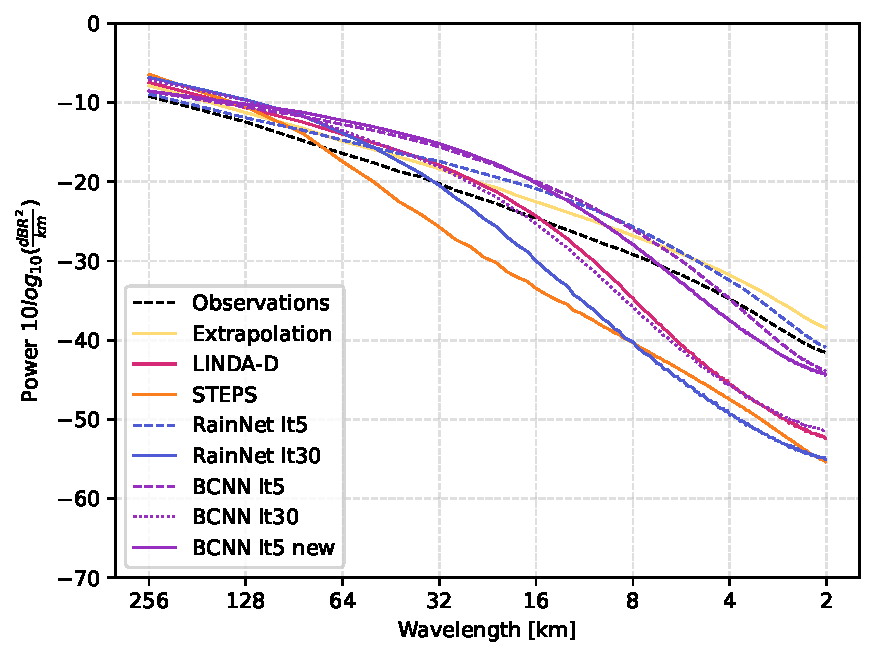
\includegraphics[width=0.33\textwidth]{images/metrics/ALL_120min_RAPSD}
	}
	\caption{Radially-averaged power spectral density (RAPSD) for BCNN variants and baselines, at leadtimes of 15 minutes, one hour, and two hours.}
	\label{fig:rapsd}
\end{figure}

\section{Probabilistic Prediction Skill}

The following section shows probabilistic prediction skill assessment results of BCNN models against STEPS and LINDA-P baselines.

\begin{figure}[H]
	\centering
	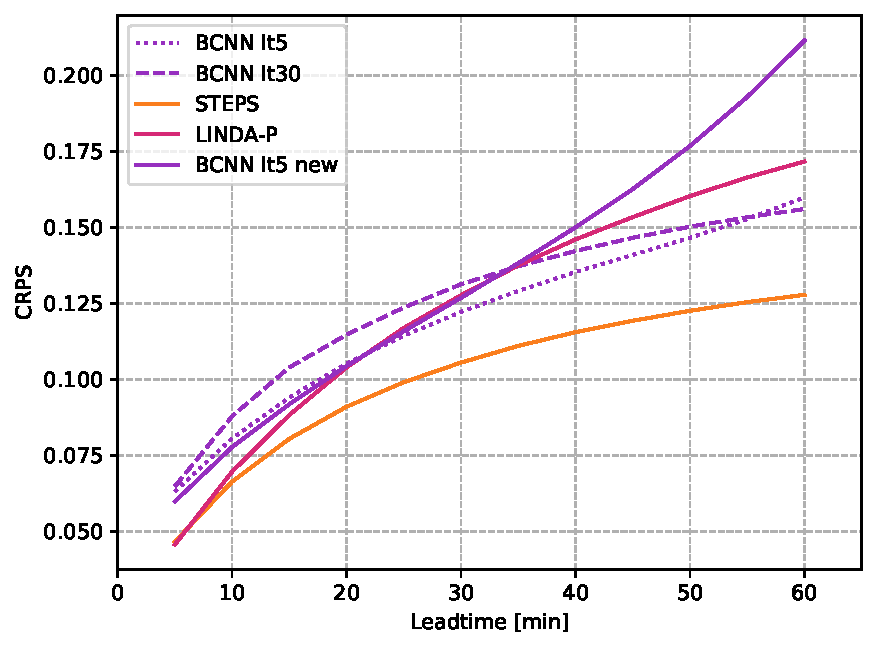
\includegraphics[width=0.6\linewidth]{images/metrics/ALL_CRPS}
	\caption{CRPS metric for all ensemble models at leadtimes up until one hour.}
	\label{fig:crps}
\end{figure}

The continuously ranked probability score for all ensemble models is shown in Figure \ref{fig:crps} for leadtimes up until one hour. Initially the best CRPS is achieved by LINDA-P, but after 10 minutes STEPS becomes the best. BCNN models consistently perform worse than STEPS, and only LINDA-P gets worse than \texttt{BCNN lt5} and \texttt{BCNN lt30} after 45 minutes.

\begin{figure}[H]
	\centering
	\subfloat[BCNN lt5]{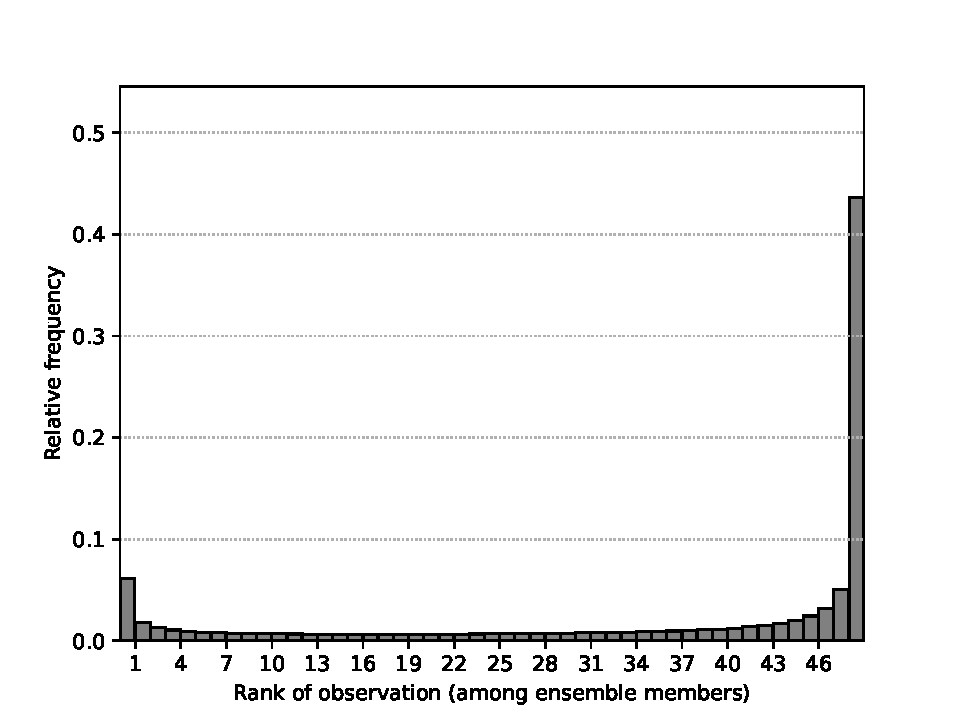
\includegraphics[width=0.5\textwidth]{images/metrics/bcnn_p2_lt5_rankhist_l_12}}%
	\subfloat[BCNN lt30]{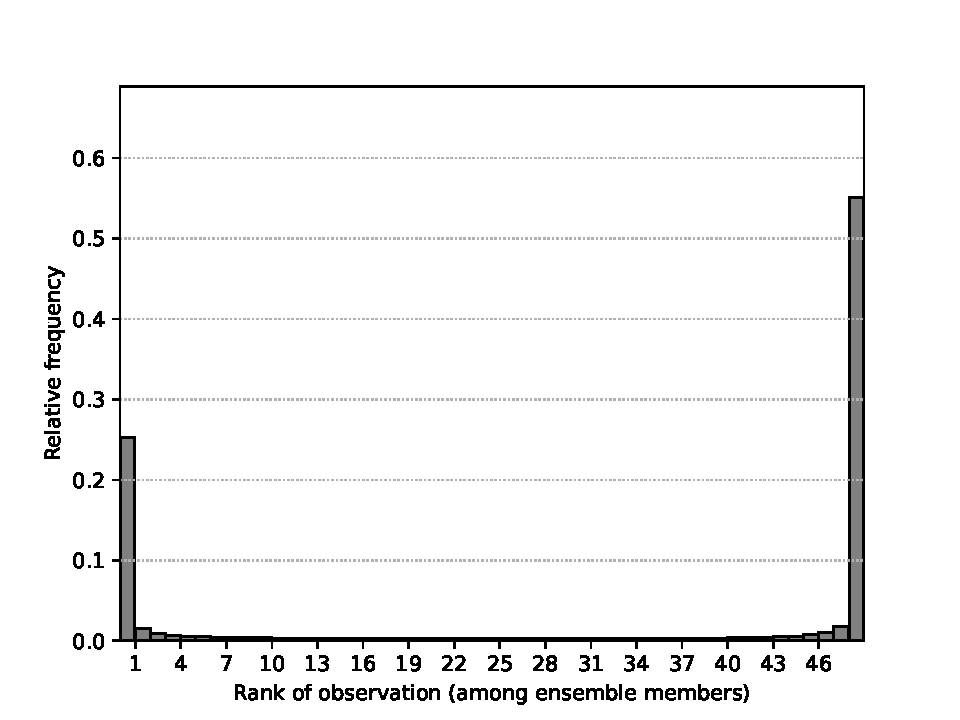
\includegraphics[width=0.5\textwidth]{images/metrics/bcnn_p2_lt30_rankhist_l_12}}%
	
	\subfloat[BCNN lt5 new]{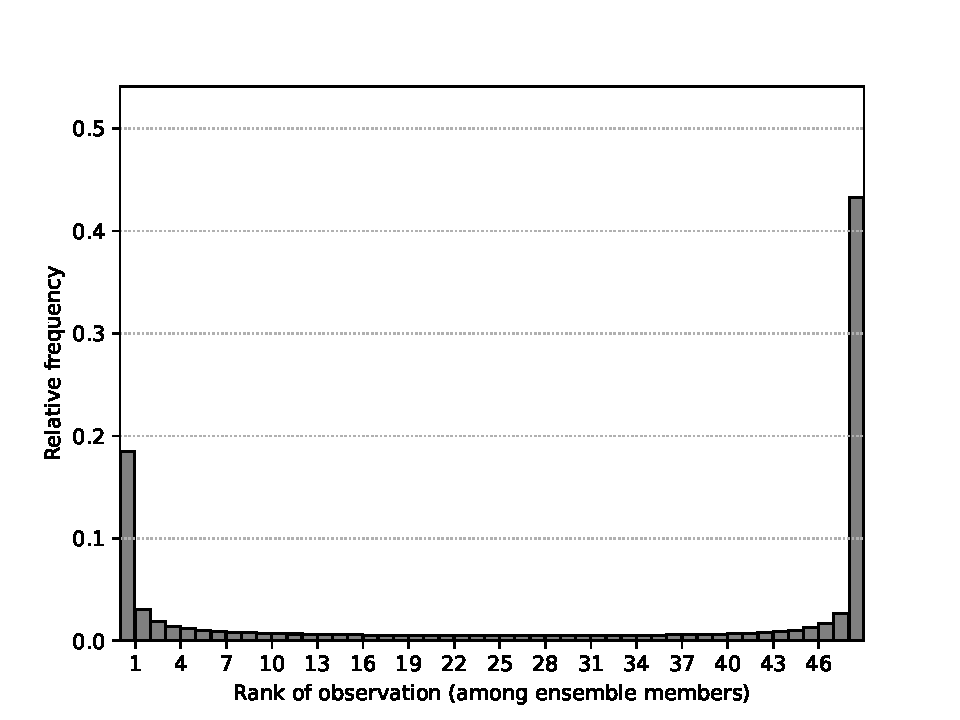
\includegraphics[width=0.5\textwidth]{images/metrics/bcnn_sdb_bs2_lt5_last_rankhist_l_12}}%
	\subfloat[STEPS]{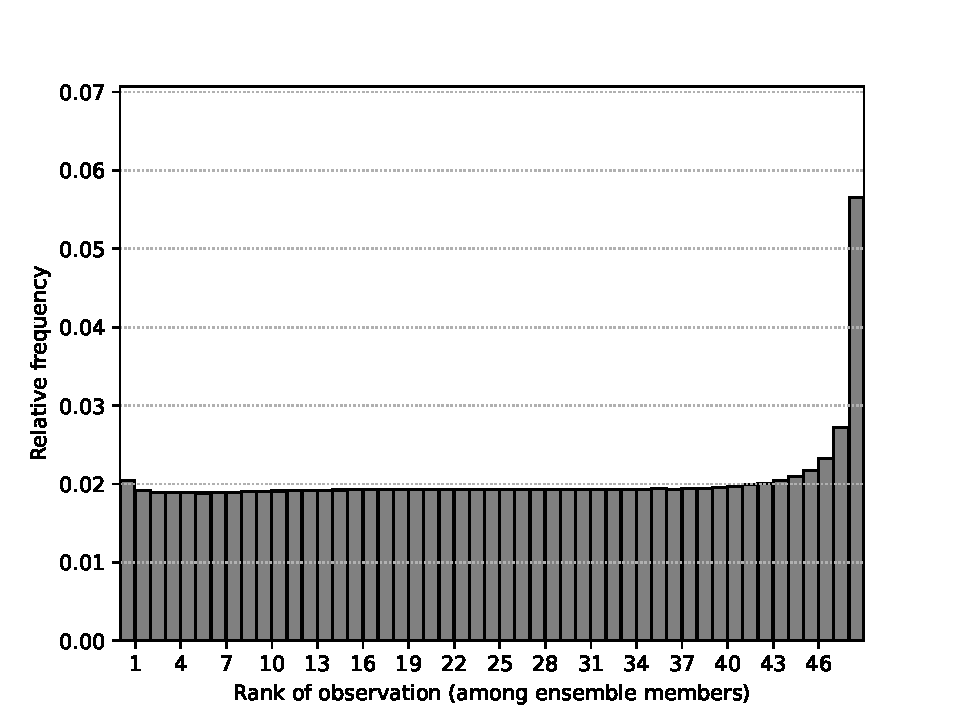
\includegraphics[width=0.5\textwidth]{images/metrics/steps_rankhist_l_12}}%
	
	\caption{Rank histograms for BCNN and STEPS model nowcasts at a one-hour leadtime, for precipitation events exceeding 0.1 mm/h.}
	\label{fig:rh}
\end{figure}

Rank histograms for BCNN and STEPS model nowcasts at one hour are shown in Figure \ref{fig:rh}, and the corresponding plot for LINDA-P is depicted in Figure \ref{fig:rankhist_linda}. It is seen that LINDA-P and especially STEPS have very flat histograms, which is indicative of well-calibrated uncertainty, i.e. no under- or over-estimation of true uncertainty is made, as observations are ranked with close to equal probability amongst ensemble members. Only a slight "negative bias" towards weak precipitation nowcasts can be detected by observing that the rightmost bin is slightly over-represented. That is cases where the observation had the highest rainrate compared to all ensemble members. 

Compared to those baselines, BCNN models had all strongly convex histograms, severely under-estimating the true uncertainty of data. Furthermore, BCNN models had the rightmost bin over-represented too, with 40 to 50\% of the time, the observation having a higher rainrate than any ensemble member. Additionally, \texttt{BCNN lt5 new} and \texttt{BCNN lt30} had around 20\% of observations where the observation was smaller than any ensemble member, hinting to many cases where the network is vastly over-confident about its high rainrate prediction. 

\begin{figure}[H]
	\subfloat[ROC 0.5 mm/h]{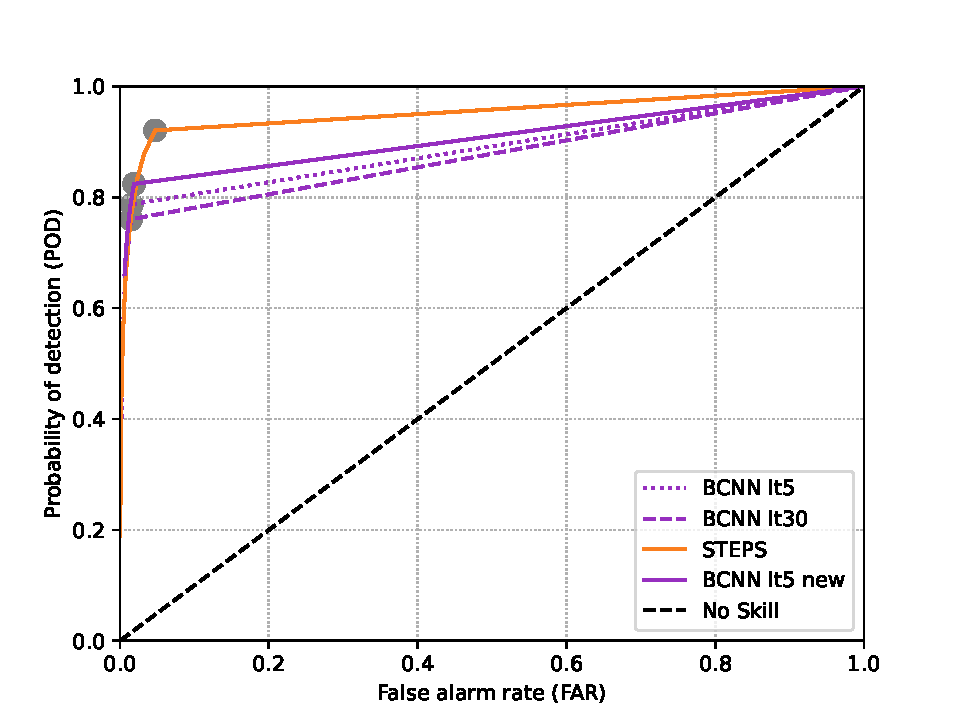
\includegraphics[width=0.33\textwidth]{images/metrics/ALL_ROC_l_12_t_0.5}}%
	\subfloat[ROC 5.0 mm/h]{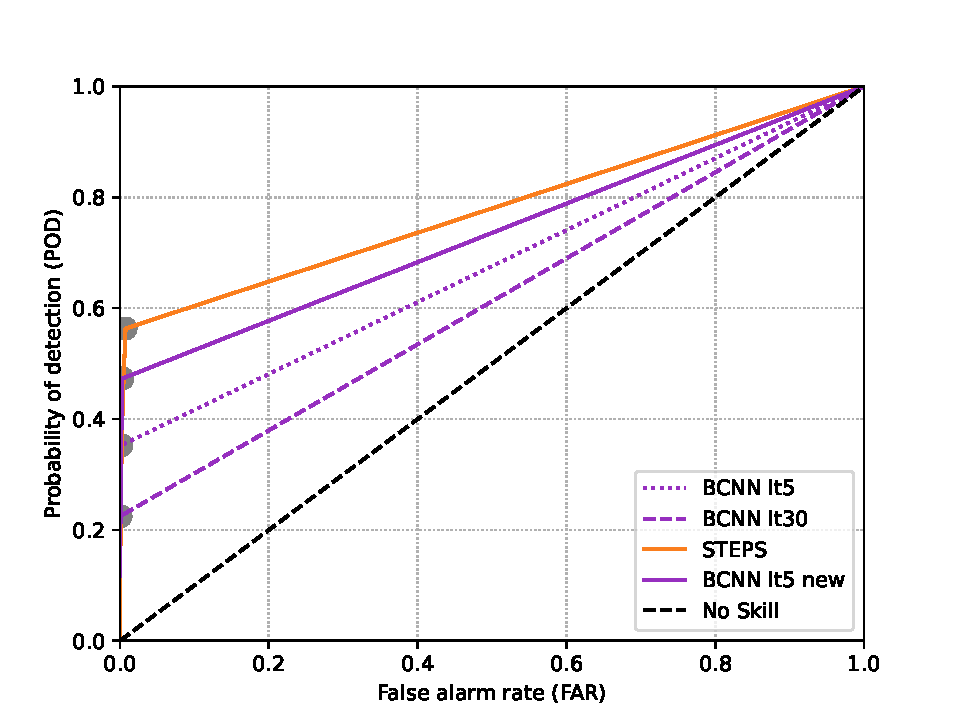
\includegraphics[width=0.33\textwidth]{images/metrics/ALL_ROC_l_12_t_5.0}}%
	\subfloat[ROC 20.0 mm/h]{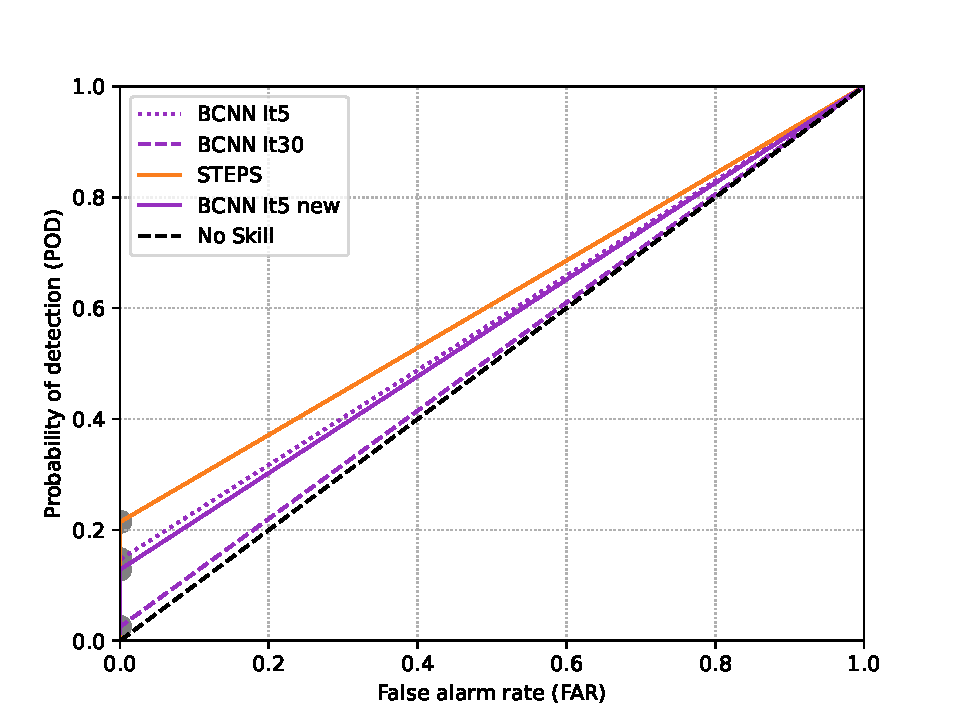
\includegraphics[width=0.33\textwidth]{images/metrics/ALL_ROC_l_12_t_20.0}}%
	
	\caption{ROC curves for one-hour exceedance probabilities at 0.5, 5.0, and 20.0 mm/h precipitation thresholds. The probability thresholds used are ten thresholds uniformly distributed between zero and one.}
	\label{fig:roc}
\end{figure}

The ROC curve for models at one hour for exceedance probabilities at thresholds of interest is shown in Figure \ref{fig:roc}, and an overview of discrimination power as a function of leadtime and threshold proxied by the ROC area under the curve (AUC) for BCNN models and STEPS is shown in Figure \ref{fig:roc_auc}. From the ROC curves, it is seen that best discriminative power is achieved by LINDA-P, overwhelmingly so at high thresholds. Second was STEPS, followed by the three BCNN models lagging far behind. From the AUC plots, it is visible that for all models, leadtime exhibits a stronger effect on discrimination power for higher thresholds. The AUC plots come to confirm that the discrimination power difference between models derived from ROC curves is consistent varying leadtime and threshold, with perhaps the exception of \texttt{BCNN lt5} compared to \texttt{BCNN lt5 new} performing better on higher, but worse on lower thresholds.

\begin{figure}[ht]
	\centering
	\subfloat[BCNN lt5]{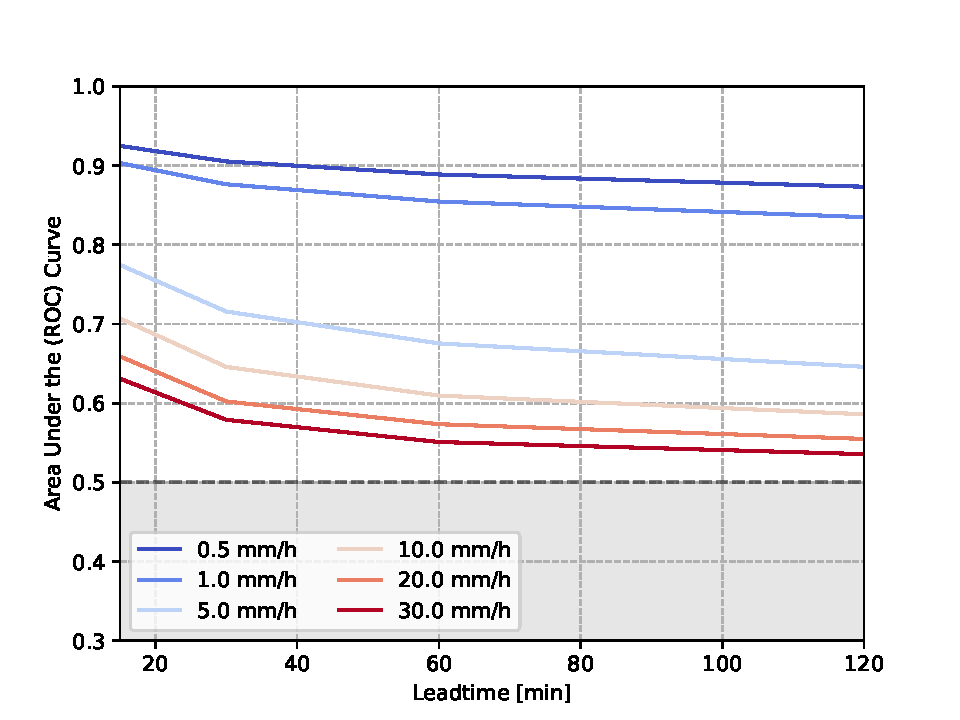
\includegraphics[width=0.5\textwidth]{images/metrics/bcnn_p2_lt5_AUC}}%
	\subfloat[BCNN lt30]{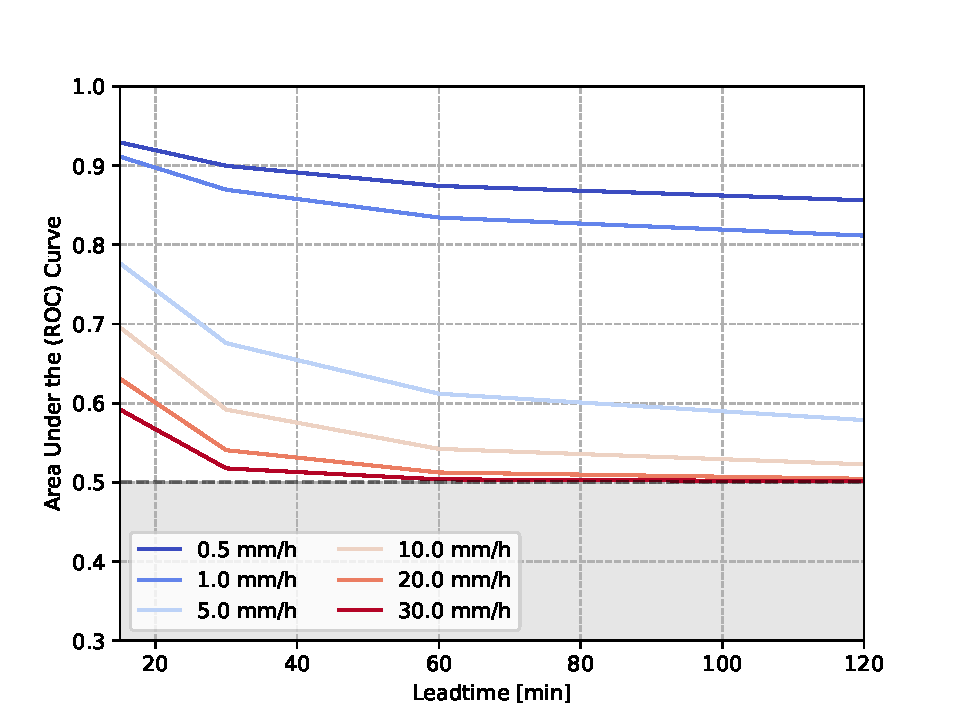
\includegraphics[width=0.5\textwidth]{images/metrics/bcnn_p2_lt30_AUC}}%
	
	\subfloat[BCNN lt5 new]{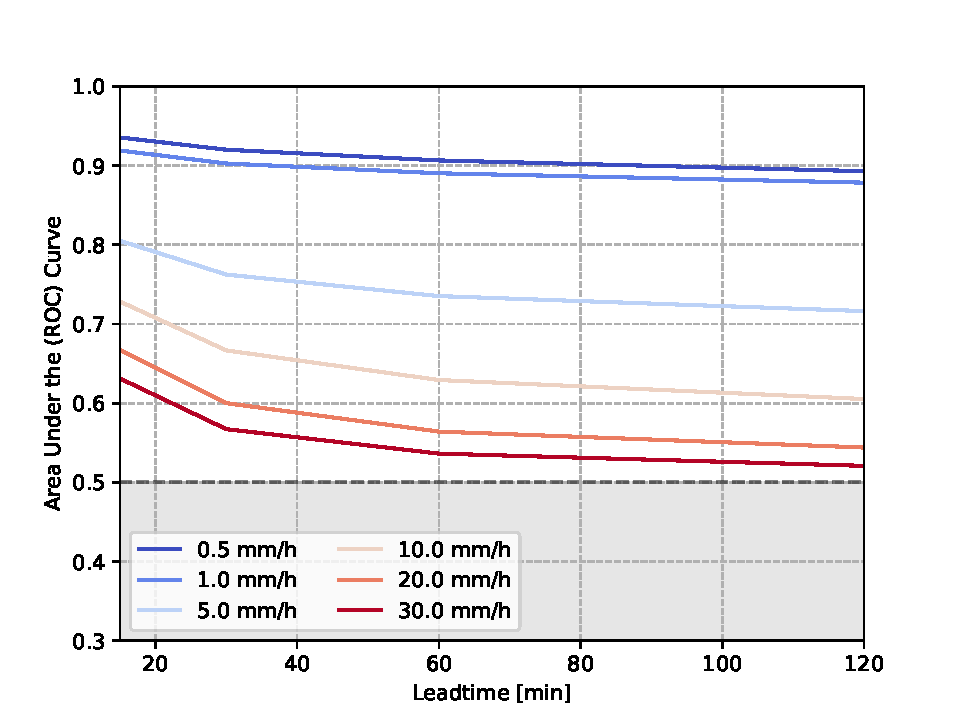
\includegraphics[width=0.5\textwidth]{images/metrics/bcnn_sdb_bs2_lt5_last_AUC}}%
	\subfloat[STEPS]{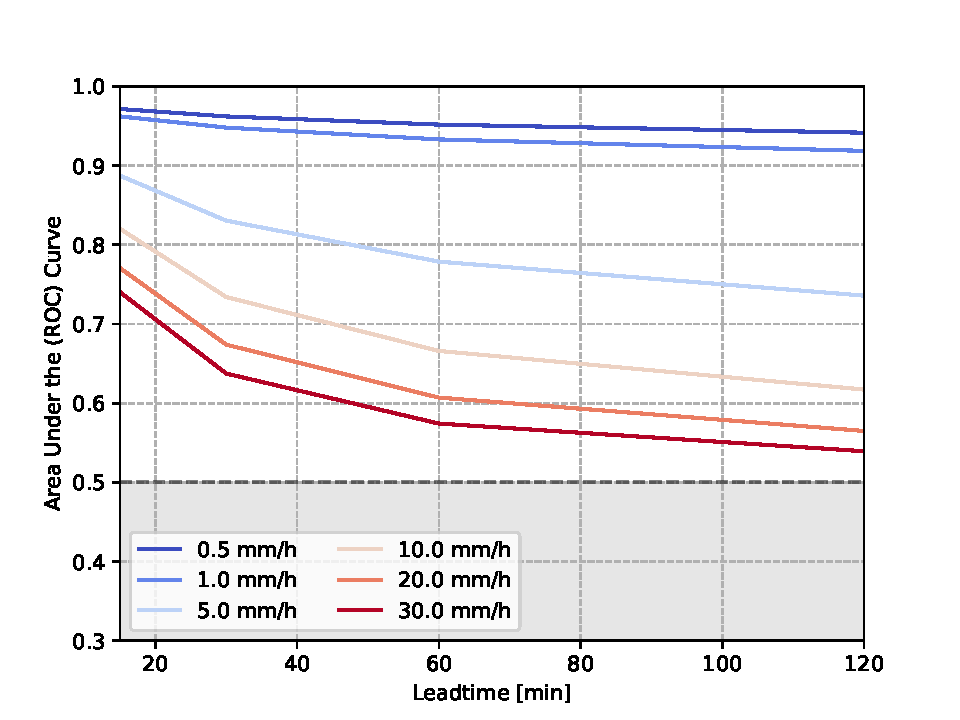
\includegraphics[width=0.5\textwidth]{images/metrics/steps_AUC}}%
	
	\caption{ROC Area under the curves summarized for BCNN and STEPS models. The dashed lines correspond to a random forecasts, and grayed out areas to results worse than that of a random (no skill) forecast.}
	\label{fig:roc_auc}
\end{figure}

Lastly, the reliability diagram accompanied by its sharpness histogram for each model, at the same precipitation thresholds at a one-hour leadtime is shown in Figure \ref{fig:reldiag}. Starting with the histogram, the sharpness of nowcasts seems to generally increase with the threshold. At 0.5 mm/h, all models have a relatively similar U-shaped sharpness histogram, indicative of moderate sharpness, with BCNN models perhaps a little sharper. Higher thresholds see all models adopt distributions of exceedance probabilities skewed towards smaller values. Generally it seems to be that it is at least one order of magnitude less common to have occurrences of forecast probabilities close to 0.5 for BCNN models compared to LINDA-P and STEPS.

Now turning towards the reliability diagram, it is clear that nowcasts get less reliable for higher thresholds. One will notice that LINDA-P and STEPS both stay both much closer to the black dashed line, indicator of perfect reliability. BCNN models tend here to assign high forecast probabilities to events that will really take place less often, and conversely assign too low forecast probabilities to events that will take place more often in practice. This expresses a lack of reliability. Furthermore, one can see that the reliability diagram of BCNN models gets non monotonous at 20.0 mm/h. This is due to too small sample sizes in the middle probabilities.

 
 \begin{figure}[H]
 	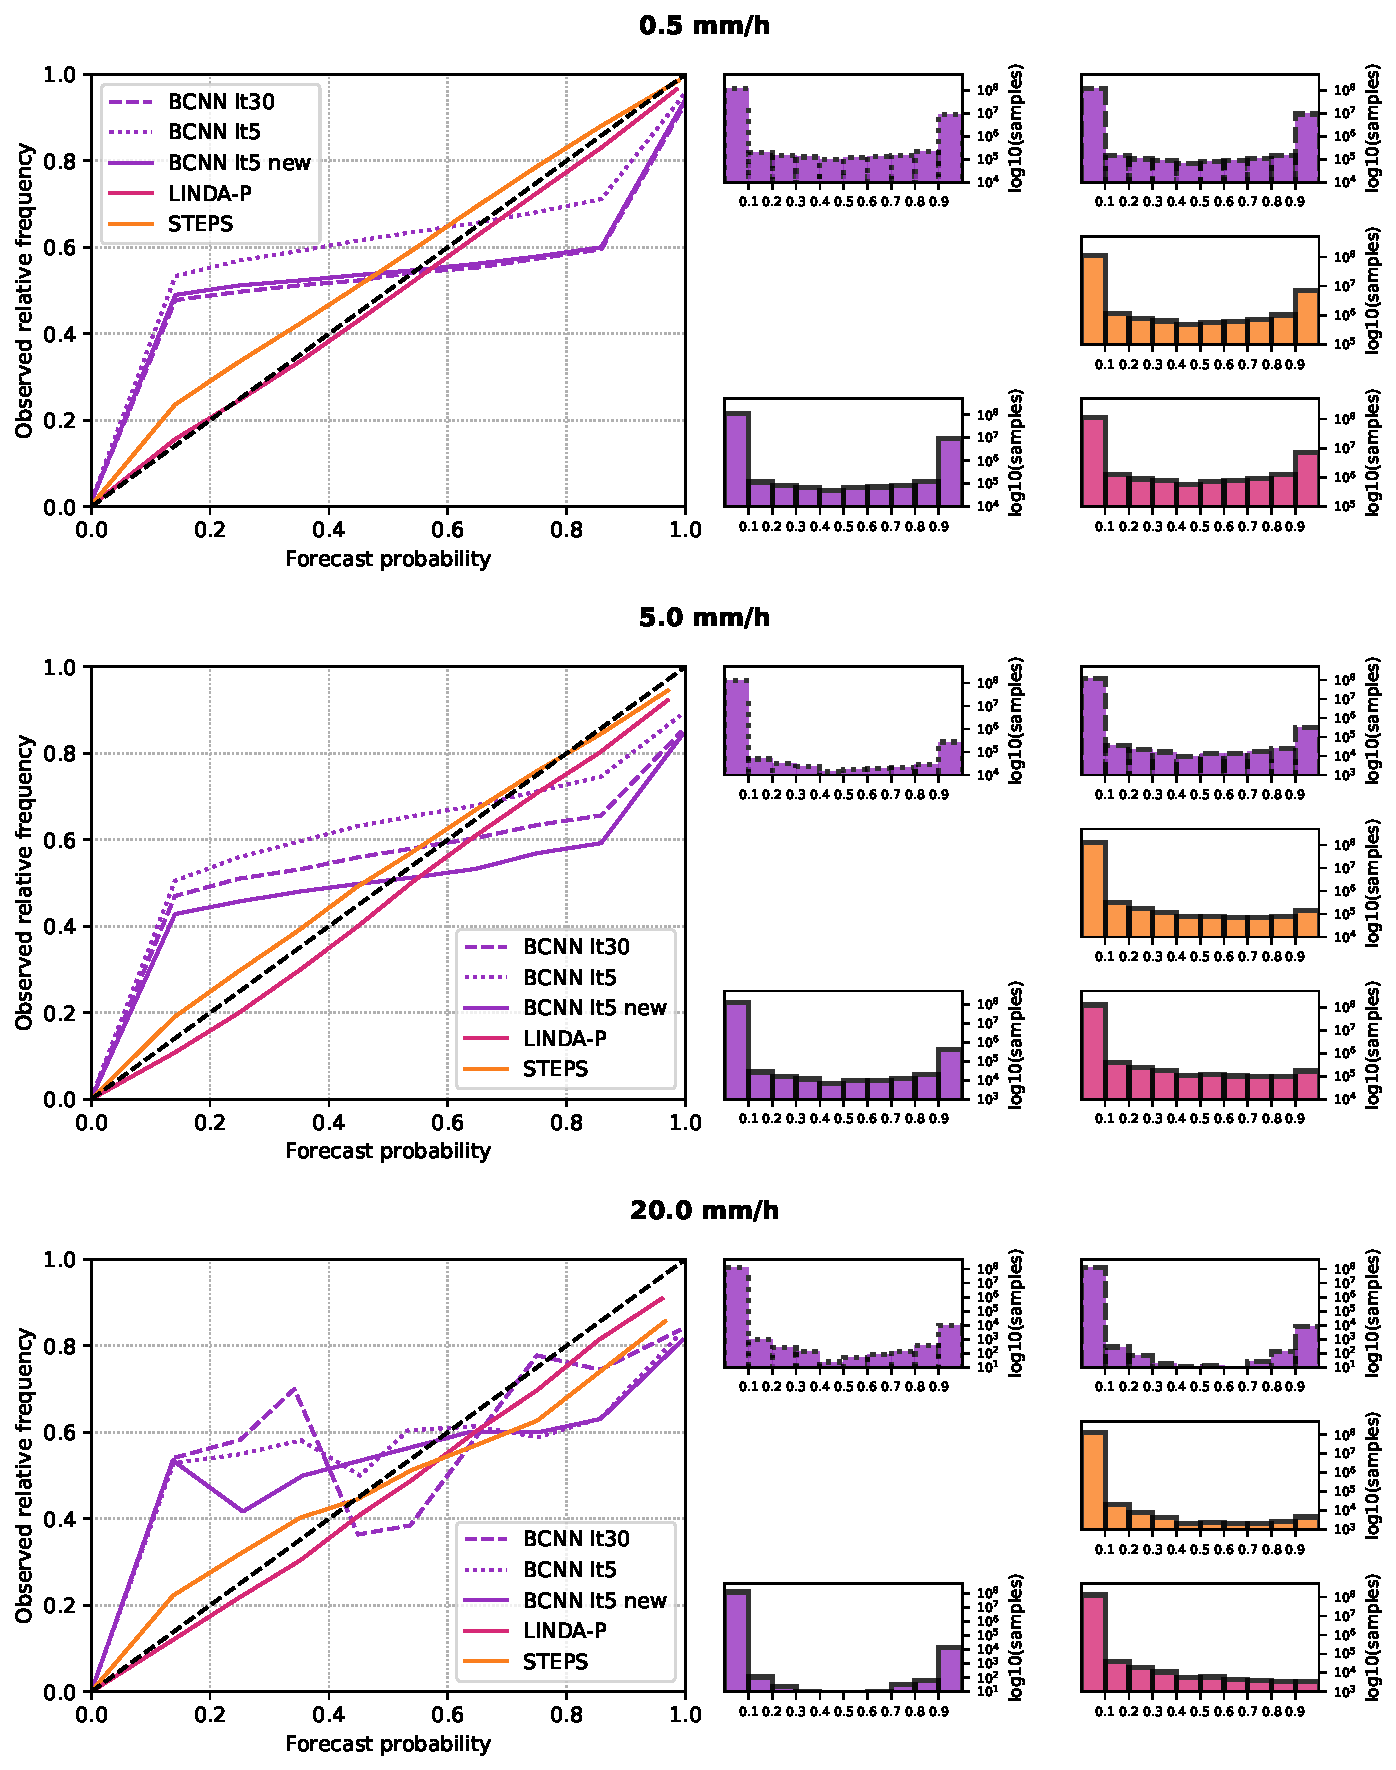
\includegraphics[width=\linewidth]{images/metrics/RELDIAG_together}
 	\caption{Reliability diagrams and sharpness histogram for one-hour exceedance probabilities at 0.5, 5.0, and 20.0 mm/h precipitation thresholds.}
 	\label{fig:reldiag}
 \end{figure}
